% This is samplepaper.tex, a sample chapter demonstrating the
% LLNCS macro package for Springer Computer Science proceedings;
% Version 2.20 of 2017/10/04
%
\documentclass[runningheads]{llncs}
%
\usepackage{graphicx}
\usepackage{url}
\usepackage{subfigure}
\usepackage{subcaption}
\usepackage{float}
\usepackage{subfloat}
\usepackage{caption}
\usepackage{mathtools}
\usepackage{array}

\begin{document}
%
\title{ATP Tennis Player Network Analysis}

\author{Kuang-Yu Li}

\institute{INFOTECH, University of Stuttgart
\email{st169971@stud.uni-stuttgart.de}}
%
\maketitle              % typeset the header of the contribution
%
\begin{abstract}
In this project, an ATP(Association of Tennis Professionals) player network 
based on tennis match statistics of ATP World Tour was built and analyzed.
The goal for this project is to discuss the correlation of several centrality rankings with 
real-world qualities of players. In the end, I landed on a conclusion that Katz centrality is the most
suitable centrality. Top 10 ranking of Katz centrality is almost aligned with the real-world evaluation of 
player. Moreover, with the comparison for different network models, the player network exhibits the 
property of scale-free network. 

\keywords{Network  \and Katz centrality \and Scale-free.}
\end{abstract}
%
%
%
\section{Introduction}
I picked this topic not only because I am big tennis fan but also because I am interested in evaluating evaluating players from the match result for the past 20 years. 
ATP stands for Association of Tennis Professionals, which is male professional tennis. ATP currently has over 1800 active players. ATP holds over 60 tennis tournaments with over 2000 matches worldwide. These tournaments are categorized into several categories according to its "points". 
Fig.~\ref{fig_example} gives an example of the point that winner can score in each tournament. Almost all tournaments are held in a single-elimination fashion. This means a player is dropped out from the tournament once he loses a match. The draw of the tournament is based on ATP ranking to separate top-ranked players from encountering each other in the early stage of tournament. With single elimination and rank-based draw, a "lucky" champion can not happen.
As mentioned above, ATP has its ranking, called ATP ranking \cite{ref_url_atp} shown in Fig.~\ref{fig_0_atp_ranking}. This ranking is also know as "world ranking". The ranking is a 52-week rolling ranking and is updated on a weekly basis. The rules of ATP ranking is only for active player. There are other ranking which focus on different aspect of player performance, such as Grand Slams ranking and GOAT points ranking \cite{ref_url_goat}. All of these rankings has its limitation.ATP ranking system only includes  active players. It is not logical to compare the retired players with active ones simply based on their rankings since they may not in the same period. For example, both Roger Federer and Andre Agassi were ranked no.1 in ATP during their prime years. I hope that by constructing a network from match statistic I could gain further insights in player evaluation. 

\begin{figure}[H]
\centering
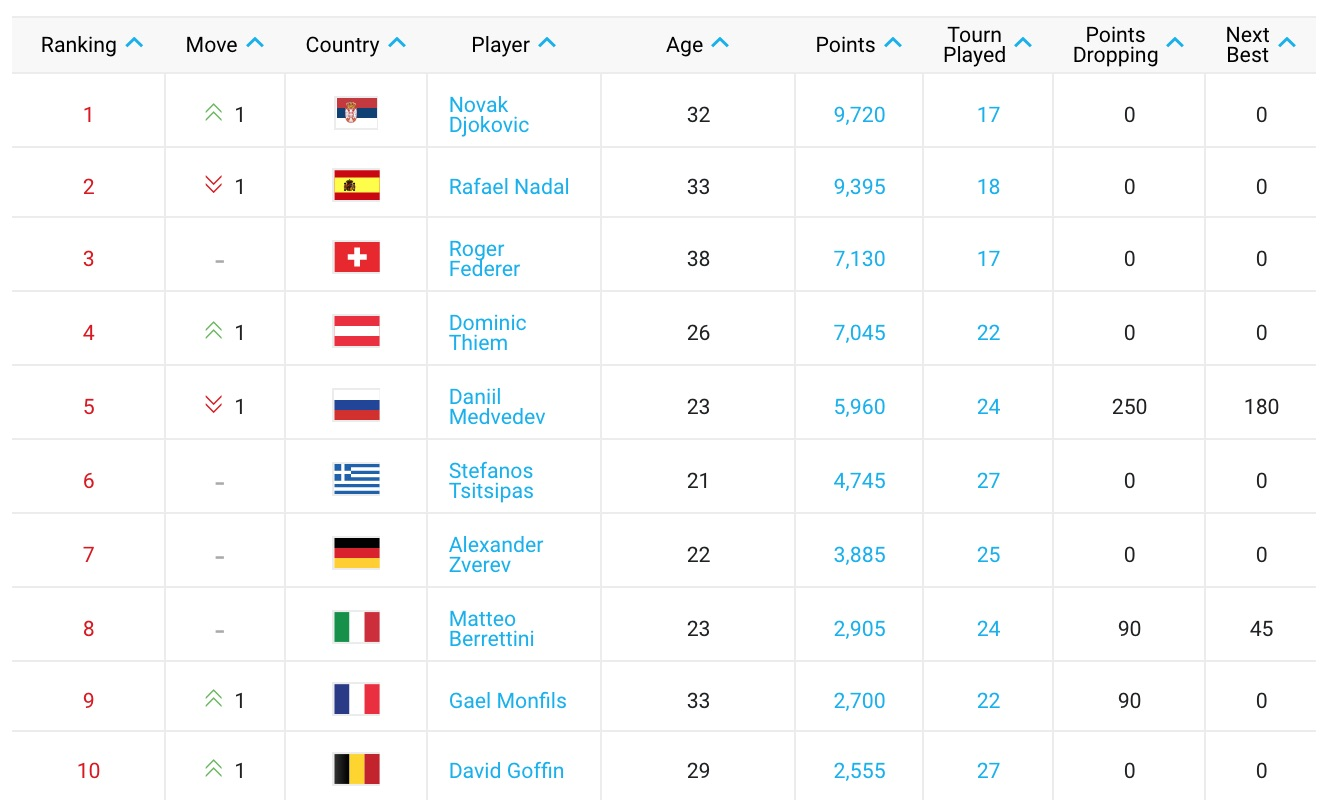
\includegraphics[scale=0.4]{ATP_ranking}
\caption{ATP ranking} \label{fig_0_atp_ranking}
\end{figure}


Real data is collected from ATP match statistic from 1996~2016. A network is constructed based on this graph. 
Each node represent a tennis player. An edge represents a match fought between two players. Each each has an attribute of "weight", indicating the total number of matches.
To simplify the analysis of network, I chose my network to be a undirected graph with weighted edge.
After constructing the network, there are 3,035 nodes and 45,563 edges

\begin{figure}[H]
\centering
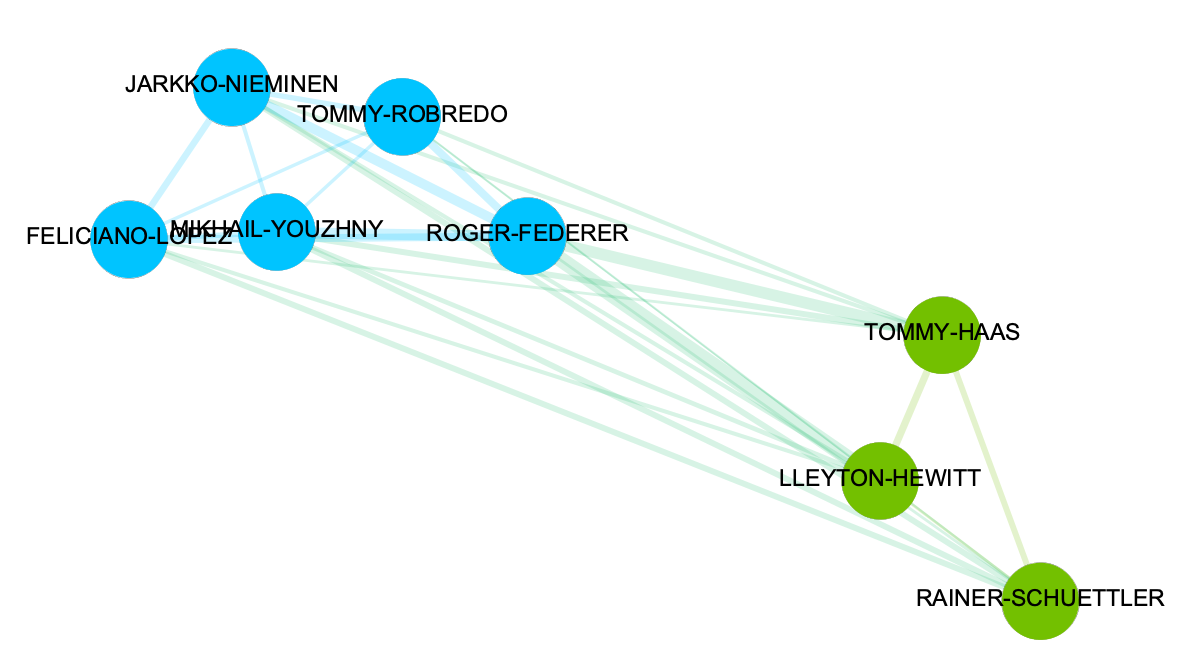
\includegraphics[scale=0.4]{0_simple_example}
\caption{An example of constructing network.} \label{fig_0_simple_example}
\end{figure}

\begin{figure}[H]
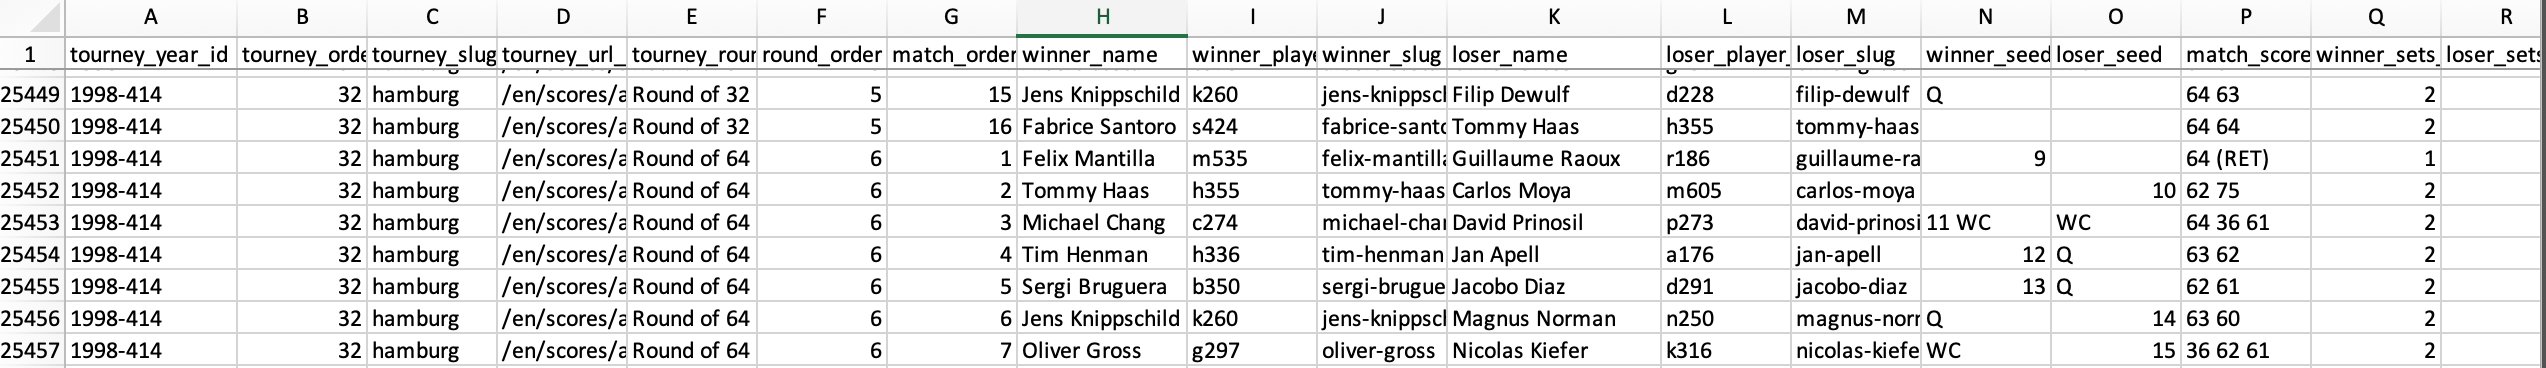
\includegraphics[width=\textwidth]{0_rawcsvdata}
\caption{Raw Data} \label{fig_rawdata}
\end{figure}


Fig.~\ref{fig_0_simple_example} gives a zoomed in part of my tennis player network.
Fig.~\ref{fig_mynk} shows the complete graph of my network.
Fig.~\ref{fig_rawdata} shows the raw data of my statistics. Using Python parsing the raw data, I parsed only the winner and loser of each match and used the data to construct my network.
Even though both winner and loser are used as node, the undirected edge cannot provide any info about how many much a player wins over another player. There are no self-loops to be removed since ,obviously, a player cannot fight against himself, unless the raw data is flawed. There are no disconnected nodes in the network. All nodes are in a single component. Analysis of the following sections are all implemented through Python and using the network analysis library NetworkX. The representation of network employs software Gephi. The source code and data can be found in \cite{ref_url1} and \cite{ref_url2}. 
From the graph of the network, a dense oval-shaped area is in the center of the graph. These are the player with higher degree, which means they are either playing many matches or constantly winning. Among these area are some of the most prominent players in the last two decades such as Roger Federer, Rafael Nadal, Pete Sampras and Andrew Agasi. The outer rim of the graph are players with only few connection with the nodes in the oval area. These players are less competitive than others. Three colors are shown to indicate to communities for each player based on modularity. We will discuss the communities in later section. In the graph, the size of a node is proportional to the number of degree. To make the big nodes prominent, the scaling of size is approximated by non-linear function.



\begin{figure}[ht]
\includegraphics[width=\textwidth]{1_graph}
\caption{Tennis Player Network 1996~2016} \label{fig_mynk}
\end{figure}


% Section Structural Insight
\todo{add other ranking graph}

\section{Structural Insight}

The structural insight basically follows the project requirement provide through the exercises.  My expectation for the network before starting analysis is as follow: 
First, the graph would be well connected with small diameter. The maximal stage of a 128-player tournament is 7. The diameter should just be a little higher than this. Second, I expected the clustering coefficient to be higher than 0.2, which is a average number from social network. Tennis player network tends to engage more than everyday social interaction. Third, the average path length is also expected to be shorter for the same reason given above. Last, I expect one of the centralities can provide a better evaluation of player in real world. With that being said, I hope one of the centrality rank cab be more representative than or comparable to the current ranking systems.
Using NetworkX, I am able to compute the structural metric for my network.
\begin{table}[H]
\centering
\caption{Structural metrics of my network.}\label{tab_my}
\begin{tabular}{|l|l|}
\hline
metric & value \\
\hline
average degree & 49.154 \\
order & 3,035 \\
size & 45,563 \\
density & 0.009896 \\
diameter & 8 \\
radius & 4 \\
average path length & 3.263307 \\
average clustering coefficient & 0.004897 \\
transitivity & 0.350256 \\
number of triangle & 745,720 \\ 
number of clique & 12,066,625 \\
number of component & 1\\
\hline
\end{tabular}
\end{table}


Table~\ref{tab_my} listed the structural metrics from my player network.
 Several things are worth mentioning here. First, number of  triangles is divided by 3 because the NetworkX function counted a triangle 3 times, each node for a time. The average clustering coefficient is the average of all local clustering coefficient. In here, the calculation of local clustering coefficient takes the weighted edge into account. The detail of formula can be found in ~\cite{ref_url_cluster_coeff} Therefore, the average clustering coefficient is not transitivity, which is derived from formula in textbook ~\cite{ref_book1}.

Both diameter, average shortest path length are low as expected. Further, the clustering coefficient is 0.35. This number is very high, compared with 0.20 in network of film actor collaborations, 0.09 in network of collaborations between biologists and 0.16 in a network of people who sends email to whom in a large university. There is only one component.

Looking further into distance distribution in Fig.~\ref{fig_2_distance_distribution_hist}, we can see that the majority of shortest path is around average 3.26 and the portion decrease drastically when shortest path increased. There are only neglectable amount of players with length over 5.

\begin{figure}[H]
\centering
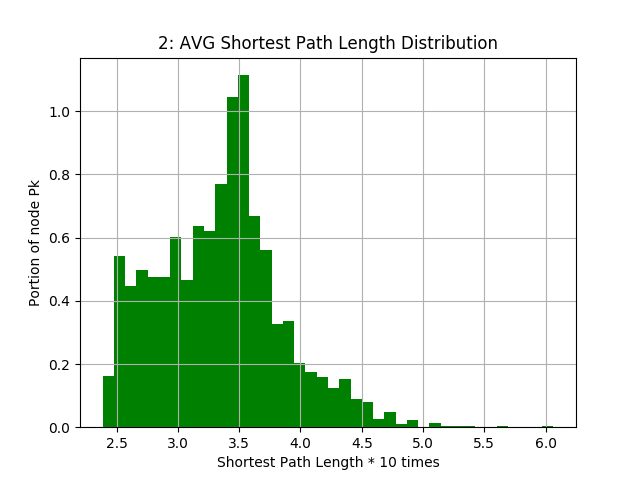
\includegraphics[scale=0.5]{2_distance_distribution_hist}
\caption{Distance Distribution} \label{fig_2_distance_distribution_hist}
\end{figure}


Histogram of degree distribution and log-scale scatter plot are shown in  Fig.~\ref{fig_2_Degree_dist_hist} and Fig.~\ref{fig_2_Degree_dist_log}. The plot behaves similarity with the scale-free network. Further comparison of my network with  a self-generated preferential attachment network will be discussed in the Network Model
 section. 
 
 \begin{figure}
    \centering
    \begin{minipage}{0.5\textwidth}
        \centering
        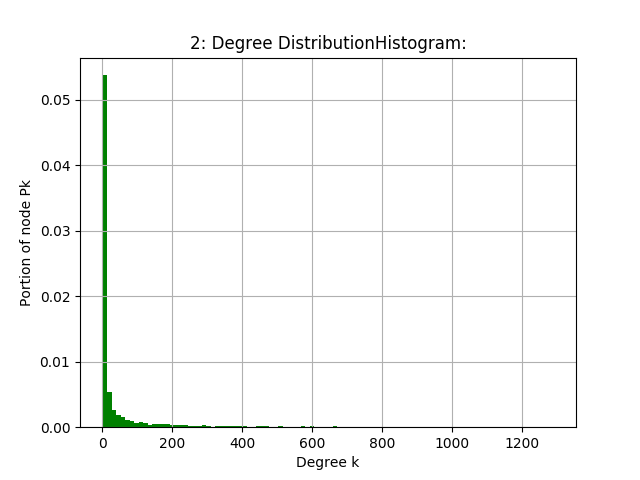
\includegraphics[width=\textwidth]{2_Degree_dist_hist} % first figure itself
        \caption{Degree dist. Histogram}
        \label{fig_2_Degree_dist_hist}
    \end{minipage}\hfill
    \begin{minipage}{0.5\textwidth}
        \centering
        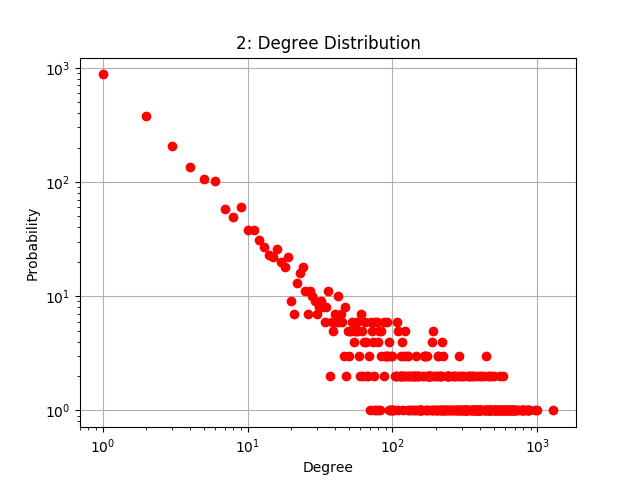
\includegraphics[width=\textwidth]{2_Degree_dist_log} % second figure itself
        \caption{Degree dist. logscale}
        \label{fig_2_Degree_dist_log}
    \end{minipage}
\end{figure}
 
Scatter plot of clustering coefficient to degree is shown in Fig.~\ref{fig_2_clustering_coeff} and Fig.~\ref{fig_2_clustering_coeff_log}. From the log-scale, we can see that the clustering coefficient is proportional to the degree. This can well be explained by the fact that the more matches a player has fought the more likely a player is good player. Therefore, good player is more prone to play with other equally good player since the match is single elimination.

\begin{figure}
    \centering
    \begin{minipage}{0.5\textwidth}
        \centering
        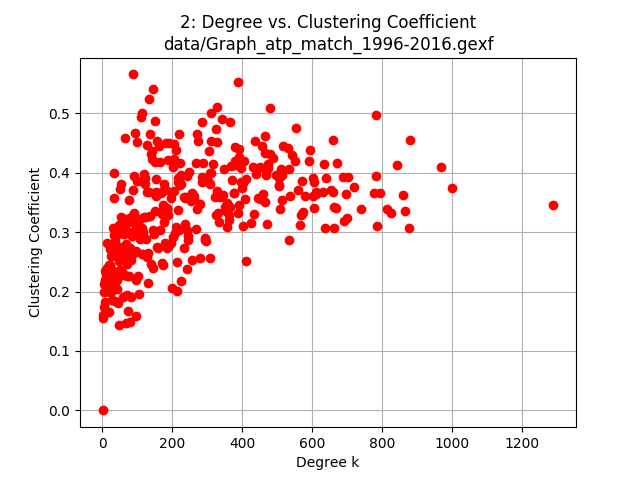
\includegraphics[width=\textwidth]{2_clustering_coeff} % first figure itself
        \caption{Clustering Coeff}
        \label{fig_2_clustering_coeff}
    \end{minipage}\hfill
    \begin{minipage}{0.5\textwidth}
        \centering
        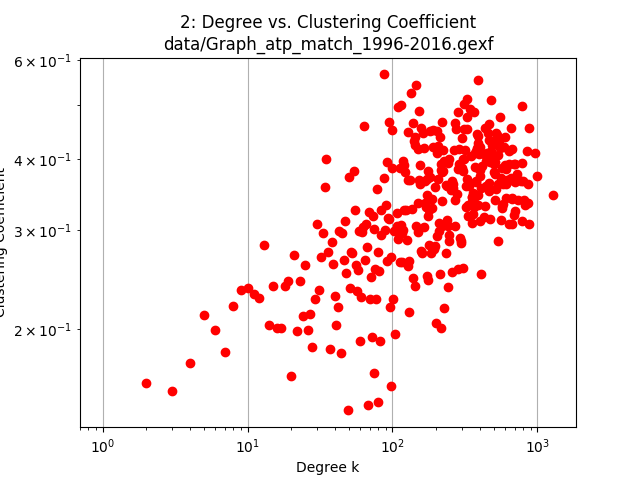
\includegraphics[width=\textwidth]{2_clustering_coeff_log} % second figure itself
        \caption{Clustering Coeff logscale}
        \label{fig_2_clustering_coeff_log}
    \end{minipage}
\end{figure}

As requested, an subgraph with node's degree higher than 10 is shown in Fig.~\ref{fig_1_subgraph}. The outer rim of the nodes are all excluded in this graph and only leaves with center oval dense area. This can well be understood that nodes in outer rim have less connection with other nodes. It reflects a large portion of players play few matches.

\begin{table}
\centering
\caption{Structural Metrics of ego network.}\label{tab_ego}
\begin{tabular}{|l|l|}
\hline
metric & value \\
\hline
order & 303 \\
size & 16,047 \\
density & 0.350731 \\
diameter & 2 \\
radius & 1 \\
average path length & 1.649269 \\ 
average clustering coefficient & 0.028295 \\ 
transitivity & 0.589713 \\ 
number of triangle & 404,647 \\ 
number of clique & 5,621,903 \\ 
number of component & 1 \\ \hline
\end{tabular}
\end{table}

An ego network for Roger Federer is constructed and is shown in Fig.~\ref{fig_2_ego_FEDERER}.Table~\ref{tab_ego} listed the structural metrics of Roger Federer ego network. Roger Federer was chosen because he ranked first in Eigen centrality, Katz centrality and Page Rank. Two noticeable metrics in this network are diameter and transitivity. The diameter becomes much smaller with the order of network significantly reduced. The transitivity becomes a lot higher, almost twice of player network. This indicates that the players fighting Federer are more likely to fight each other. It actually makes sense. Given that Federer is top-ranked player, the players fighting Federer may be more likely to be top ranked.

\begin{figure}[H]
\centering
\includegraphics[scale=0.05]{1_subgraph}
\caption{Subgraph with degree larger than 10} \label{fig_1_subgraph}
\end{figure}

\begin{figure}[H]
\centering
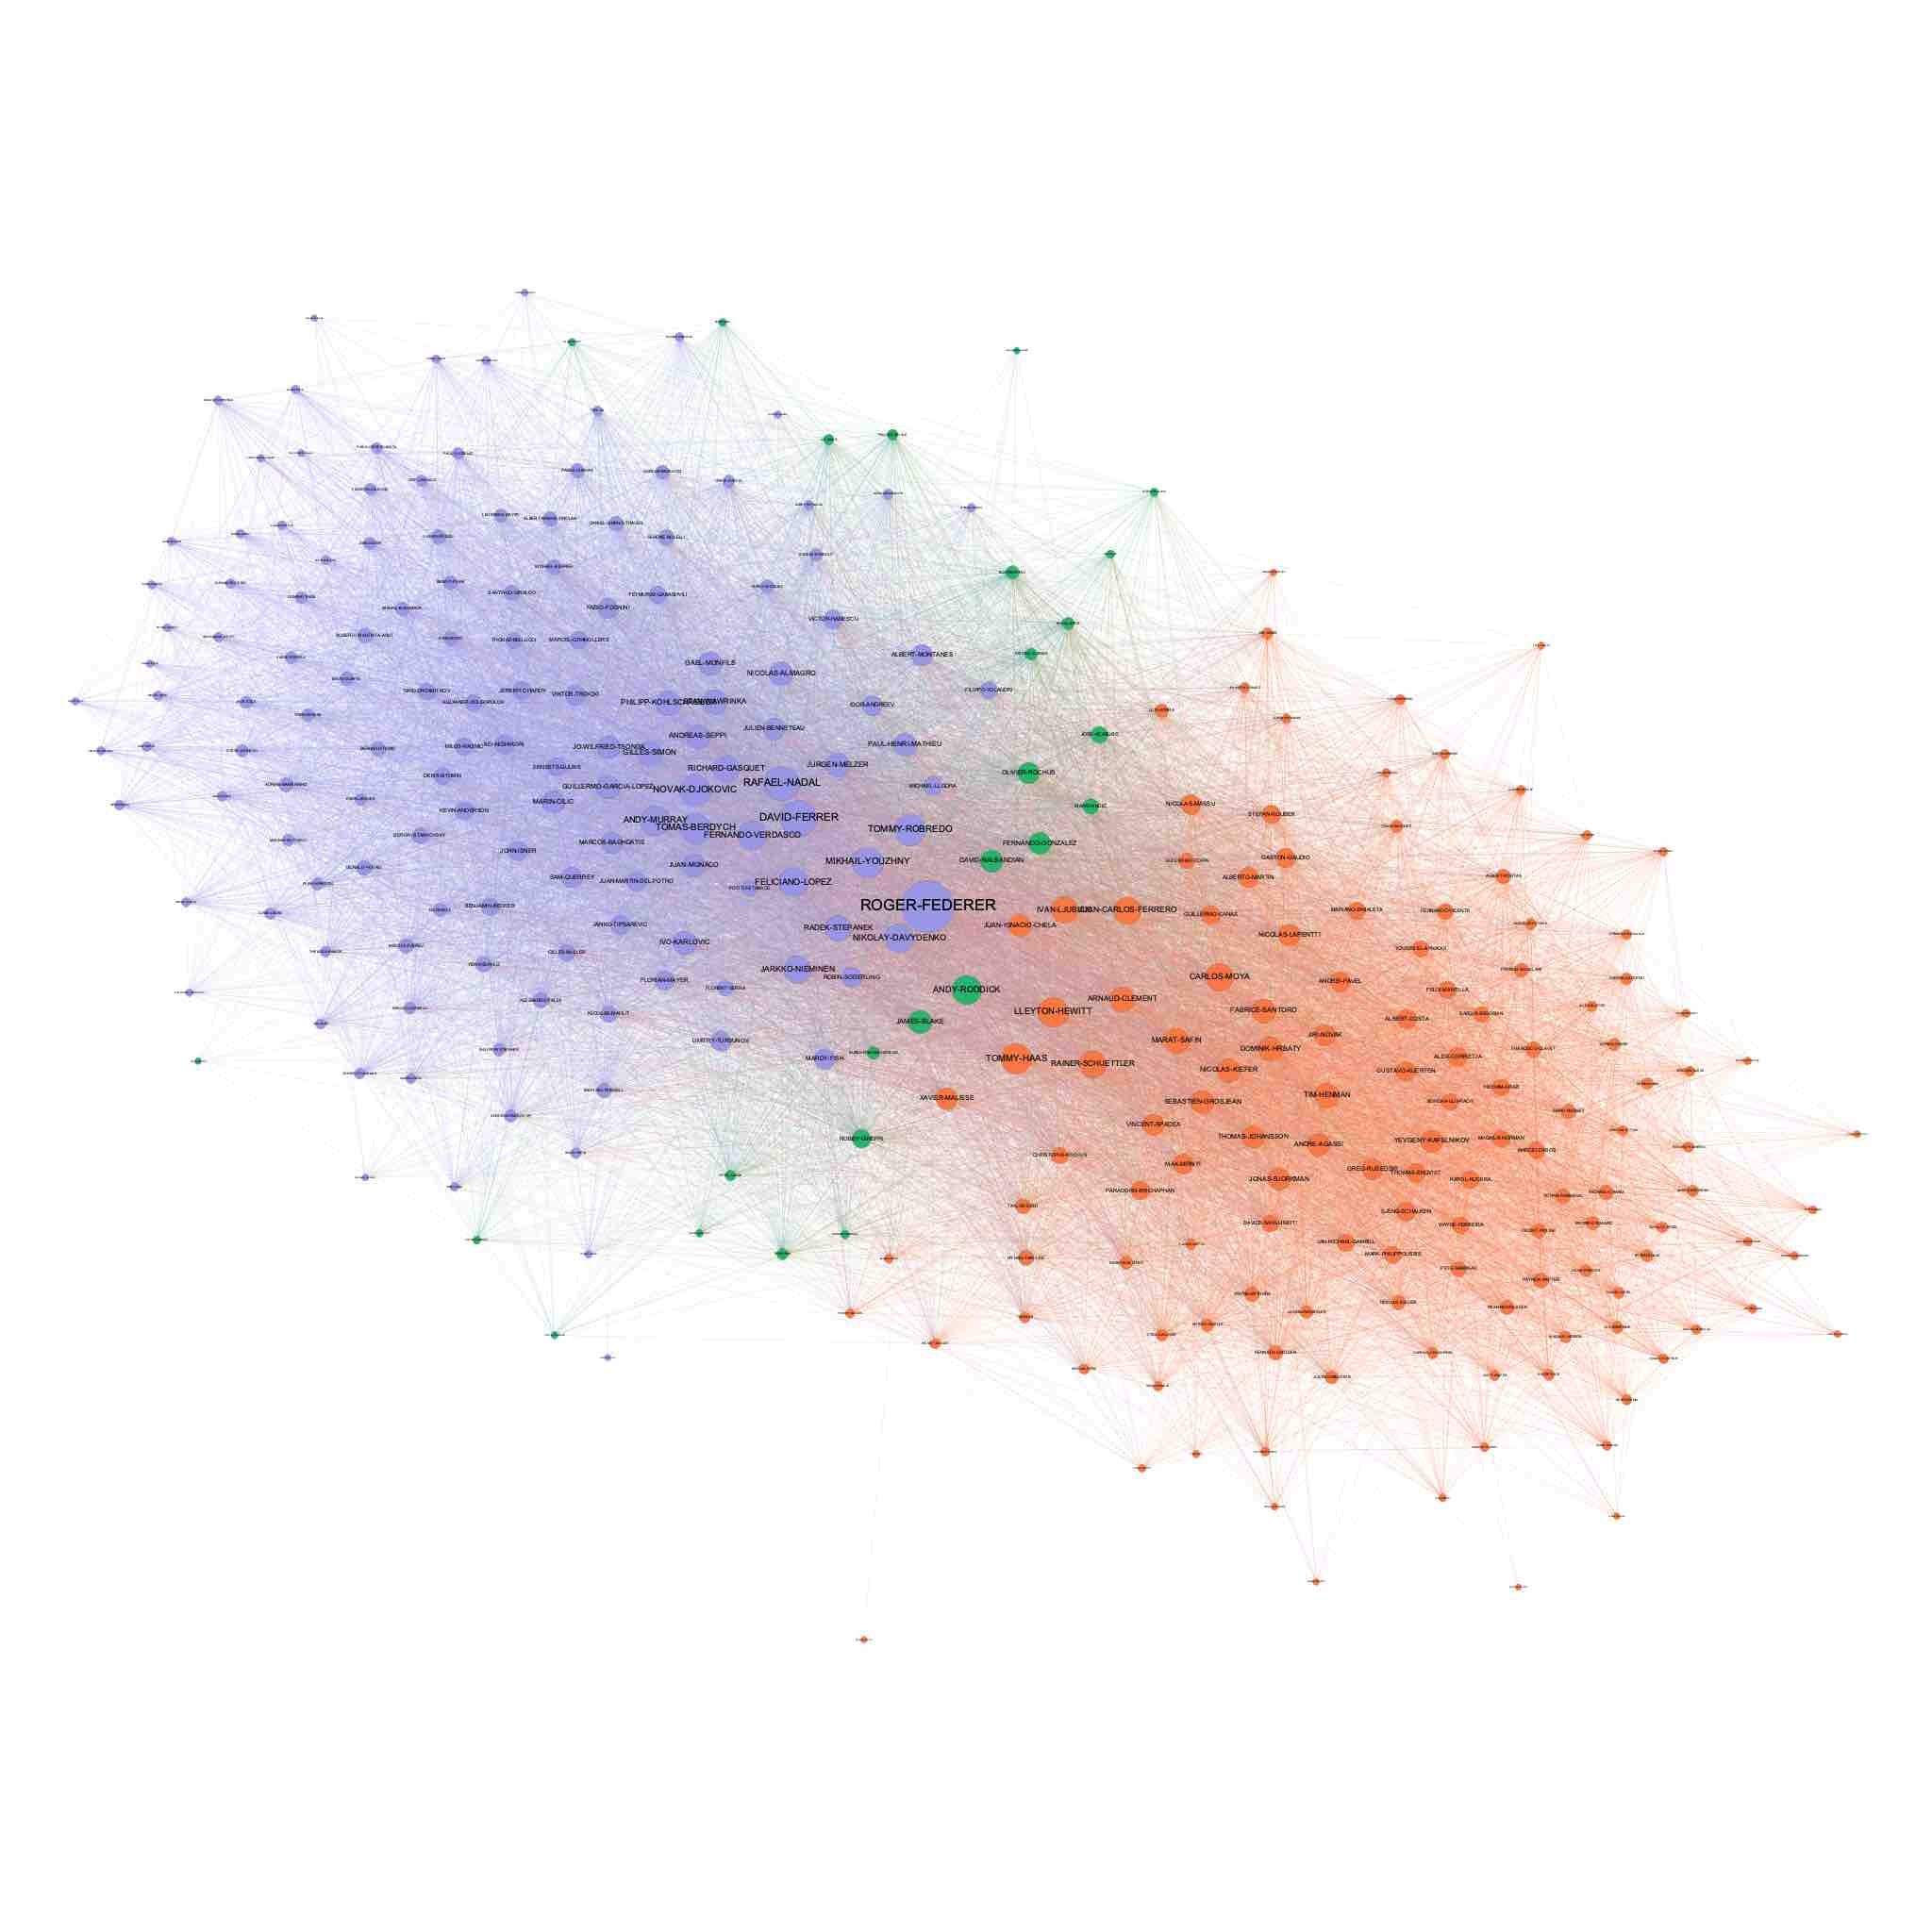
\includegraphics[scale=0.1]{2_ego_FEDERER}
\caption{Federer Ego Network} \label{fig_2_ego_FEDERER}
\end{figure}

In both player network and subgraph, three colors are presented to indicate community. This is done based on modularity function in Gephi. Why there are three big communities can be further explained through looking "big" nodes in their own community. Fig.~\ref{fig_2_player_pos} points out some of the important node in each community. I make a calculation of number of nodes in each community. It turns out that the green community comprises of 9\% of all nodes, the blue 22 \%, and the purple 67 \%. After pointing out the important/typical player of each community, I landed on a explanation for these three communities. The green community represents players who have an early retirement. Sampras and Agasi are typical example of this community.The blue community represents players who are both good and enjoys a long career. Federer, Nadal and Štěpánek makes typical examples. The purple community represents players who are somewhat ok but also enjoys a long career. Mischa Zverev and Rajeev Ram are examples. This is why the blue community is in between purple and green ones because players who retires early would not have a chance to fight newly-joined or currently-active players. Moreover, we can also conclude that young players will certainly not in the green community. He will belongs to blue community if he is a good player. Dominic Thiem is a good example for this case. The dashed line shown in Fig.~\ref{fig_2_player_pos} can roughly used to separate good players with mediocre players. I prefer to call it the "competitive oval." Players inside the oval span across all three community. The further insight of these players will be discussed in later section.




\begin{figure}[H]
\centering
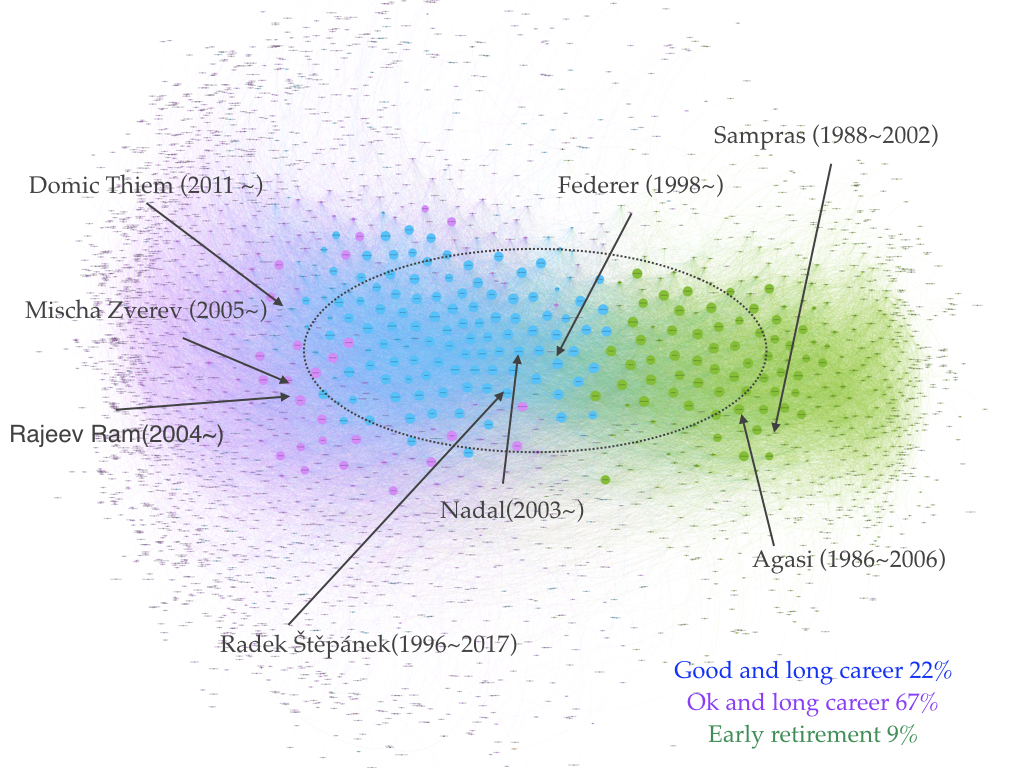
\includegraphics[width=\textwidth]{2_player_pos}
\caption{Federer Ego Network} \label{fig_2_player_pos}
\end{figure}

\begin{figure}[H]
    \centering
    \begin{minipage}{0.5\textwidth}
        \centering
        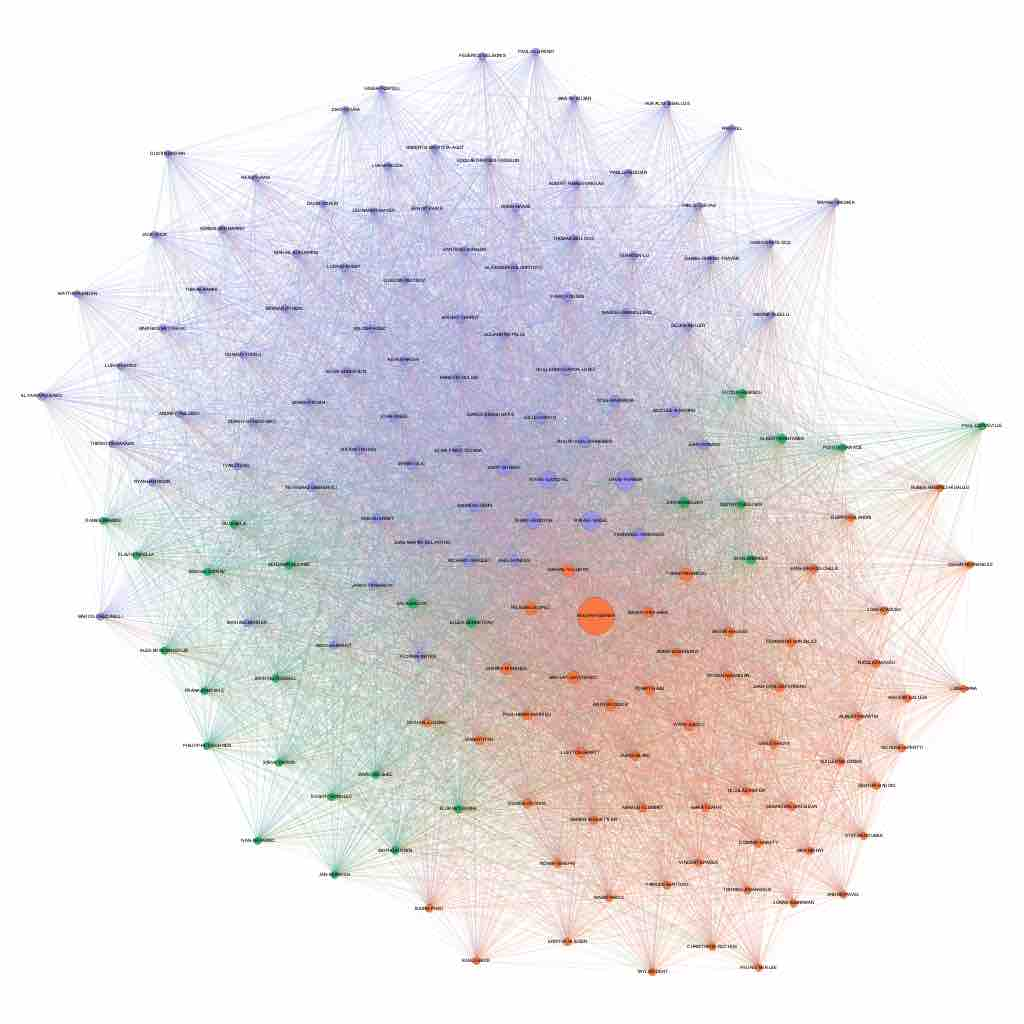
\includegraphics[width=\textwidth]{2_k_core_my} % first figure itself
        \caption{78-Core Graph}
        \label{fig_2_k_core_my}
    \end{minipage}\hfill
    \begin{minipage}{0.5\textwidth}
        \centering
        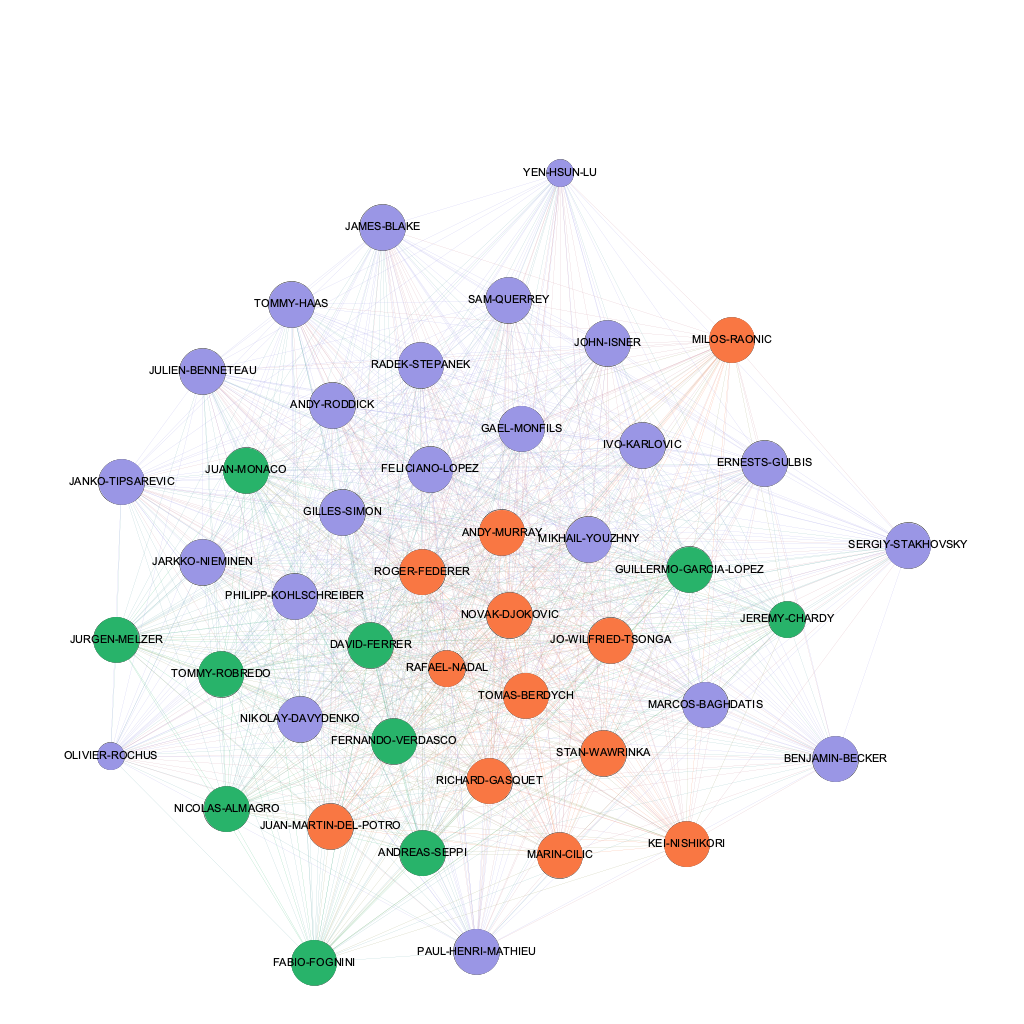
\includegraphics[width=\textwidth]{2_max_clique} % second figure itself
        \caption{Maximal Clique}
        \label{fig_2_max_clique}
    \end{minipage}
\end{figure}

A 78-core graph is shown in Fig.~\ref{fig_2_k_core_my} and its structural metrics is shown in Table.~\ref{tab_ego}. 78-core is the largest core found in my player network. As requested, I implemented the process of finding k-core myself and compared the result from the k-core from NetworkX narrative function. In the end, two functions come up with the exact result. The k-core implementation code can be found in the source code.
\todo{adding source code citation}
The transitivity is over 0.7. This is very logical due to the definition of core.
A graph consists of 3 maximal cliques shown inFig.~\ref{fig_2_max_clique} and its structural metrics is shown in Table~\ref{tab_kcore}. Three maximal cliques are found in total, each with 43 nodes.

\begin{table}[H]
\centering
\caption{Structural Metrics of k-core network.}\label{tab_kcore}
\begin{tabular}{|l|l|}
\hline
metric & value \\
\hline
order & 162 \\
size & 8954 \\
density & 0.686604 \\
diameter & 2 \\
radius & 2 \\
average path length & 1.313396 \\
average clustering coefficient & 0.039433 \\
transitivity & 0.744889 \\
number of triangle & 252,986 \\
number of clique & 6,800,942 \\
number of component & 1 \\
\hline
\end{tabular}
\end{table}



 % Centrality Insight
 
\section{Centrality Insight}

In this section, 6 different kinds of centralities are discussed. Katz centrality and Eigen centrality are the most aligned with real-world ranking. All of the centralities are calculated by the adoption of NetworkX's native functions with weighed edge enabled. The harmonic centrality is calculated from the normalized result of harmonic function. The normalization is computed by dividing node order minus one. The poor performance of Eigen centrality in directed networks is another reason I decided to make the tennis player network an undirected graph.

\begin{table}
\caption{Harmonic vs Betweenness vs Degree}\label{tab_total_compare}
\begin{tabular}{|l|l|l|l|l|l|l|} \hline
\(\#\) & Harmonic & \(H_{i}\)  & Betweenness & \(B_{i}\) & Eigen & \(k_{i}\) \\ \hline
1 & JAN-HERNYCH & 0.458 & RAJEEV-RAM & 0.016 & TOMMY-HAAS & 0.106 \\ \hline
2 & RAJEEV-RAM & 0.453 & MISCHA-ZVEREV & 0.016 & ROGER-FEDERER & 0.1 \\ \hline
3 & MICHAEL-BERRER & 0.449 & MICHAL-PRZYSIEZNY & 0.016 & MIKHAIL-YOUZHNY & 0.098 \\ \hline
4 & SIMONE-BOLELLI & 0.449 & ANDREY-GOLUBEV & 0.012 & RAINER-SCHUETTLER & 0.098 \\ \hline
5 & ANDREY-GOLUBEV & 0.449 & SERGIY-STAKHOVSKY & 0.012 & JARKKO-NIEMINEN & 0.098 \\ \hline
6 & VICTOR-HANESCU & 0.449 & GEORGE-BASTL & 0.012 & LLEYTON-HEWITT & 0.098 \\ \hline
7 & BJORN-PHAU & 0.448 & MICHAEL-BERRER & 0.012 & FELICIANO-LOPEZ & 0.097 \\ \hline
8 & MISCHA-ZVEREV & 0.448 & JAN-HERNYCH & 0.011 & TOMMY-ROBREDO & 0.097 \\ \hline
9 & TEYMURAZ-GABASHVILI & 0.448 & RUBEN-RAMIREZ-HIDALGO & 0.011 & RADEK-STEPANEK & 0.095 \\ \hline
10 & RADEK-STEPANEK & 0.446 & BJORN-PHAU & 0.01 & CARLOS-MOYA & 0.095 \\ \hline

\end{tabular}
\end{table}

Table~\ref{tab_total_compare} shows top 10 of the comparison for three centrality: Harmonic, Betweenness and Degree. There are a great similarity between Harmonic and Betweenness centrality. However, the rank of Degree centrality disagree with the other centrality. How do we explain this? We can start by looking up the names of the players. Jan Hernych is active player, turned pro in 1998 and achieved his career-high singles ranking of World No. 59 in April 2009. Rajeev Ram is also active is active, , turned pro in 2004 and achieved his career-high singles ranking of World No. 56 in April 2016. Both of them are once high ranked players and enjoy long career. They are not top skilled player. But over the course of their career, they have fought with a lots of players. We can look into Fig.~\ref{fig_3a_betweenness_centrality} and Fig.~\ref{fig_3a_harmonic_centrality} for more insights. As we can see, marked red nodes are the top 10 nodes in each centrality ranking and these nodes tend to be spread just the outer side of "competitive" oval. They are located in a position just to each other player with comparative short path. Namely, the ranking of Harmonic and Betweenness centrality reflects more about players career length rather their skill.

\begin{figure}
\centering
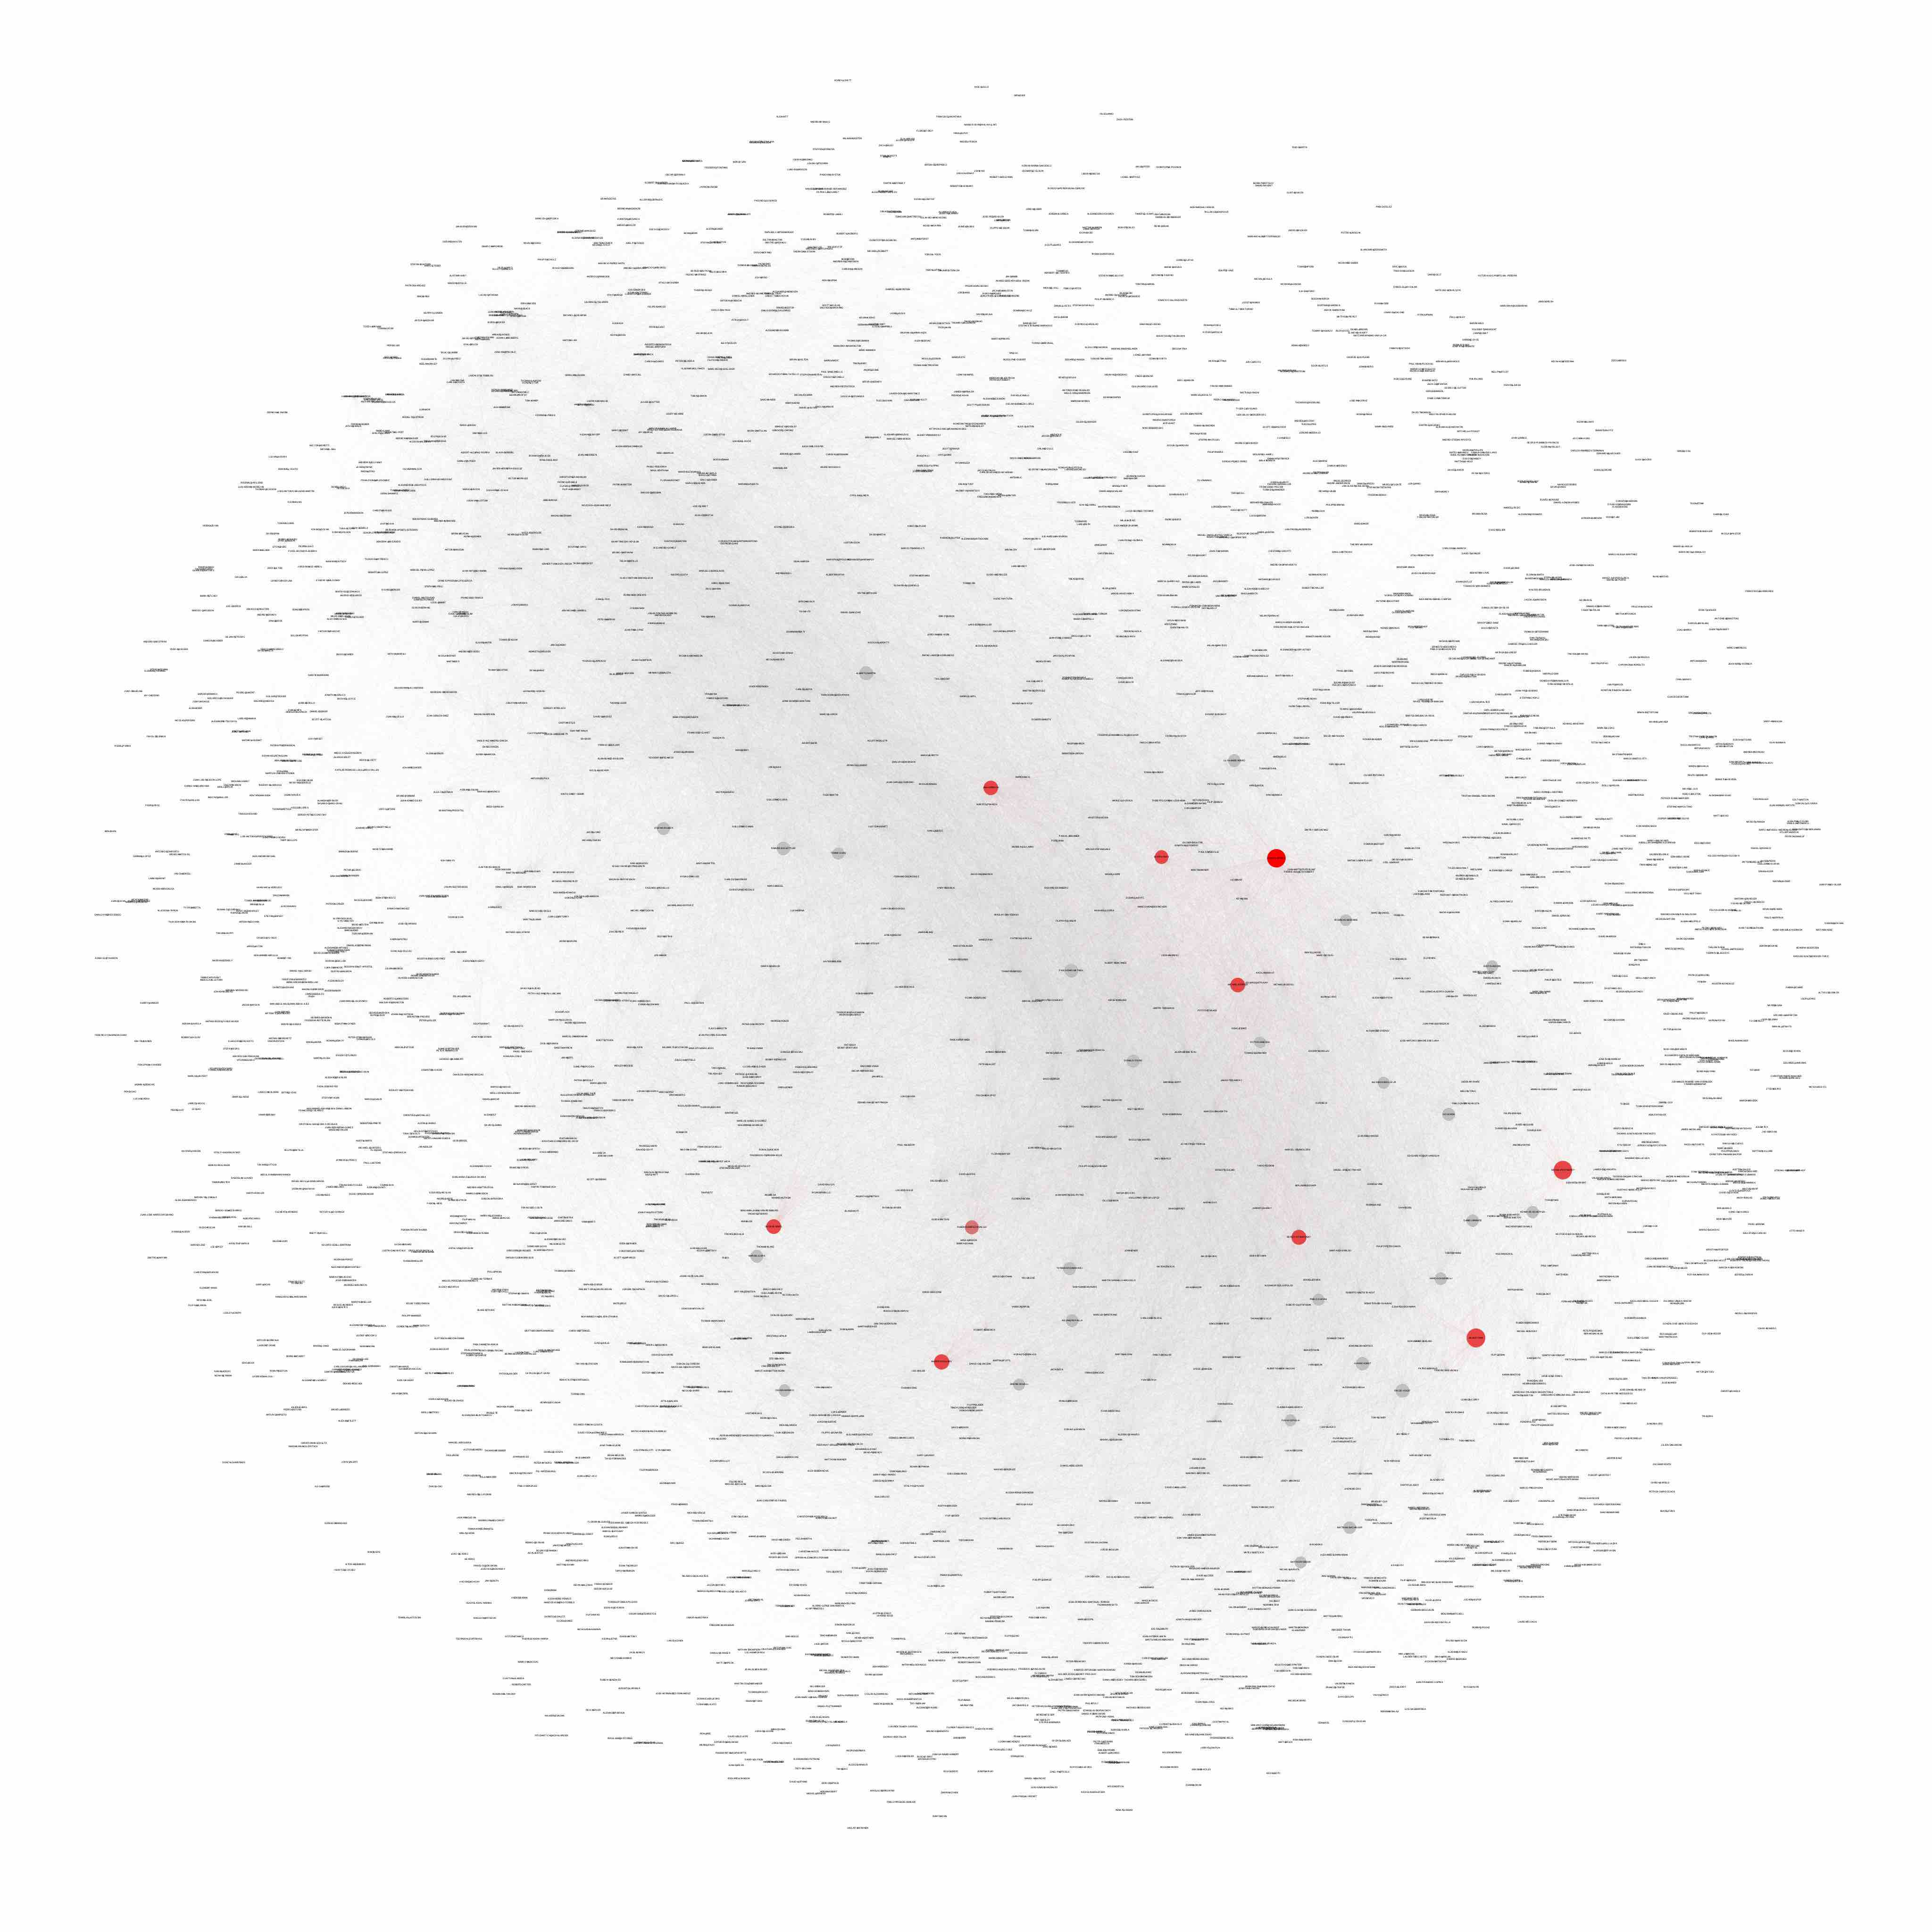
\includegraphics[width=\textwidth]{3a_betweenness_centrality}
\caption{Betweenness Centrality in network} \label{fig_3a_betweenness_centrality}
\end{figure}

\begin{figure}
\centering
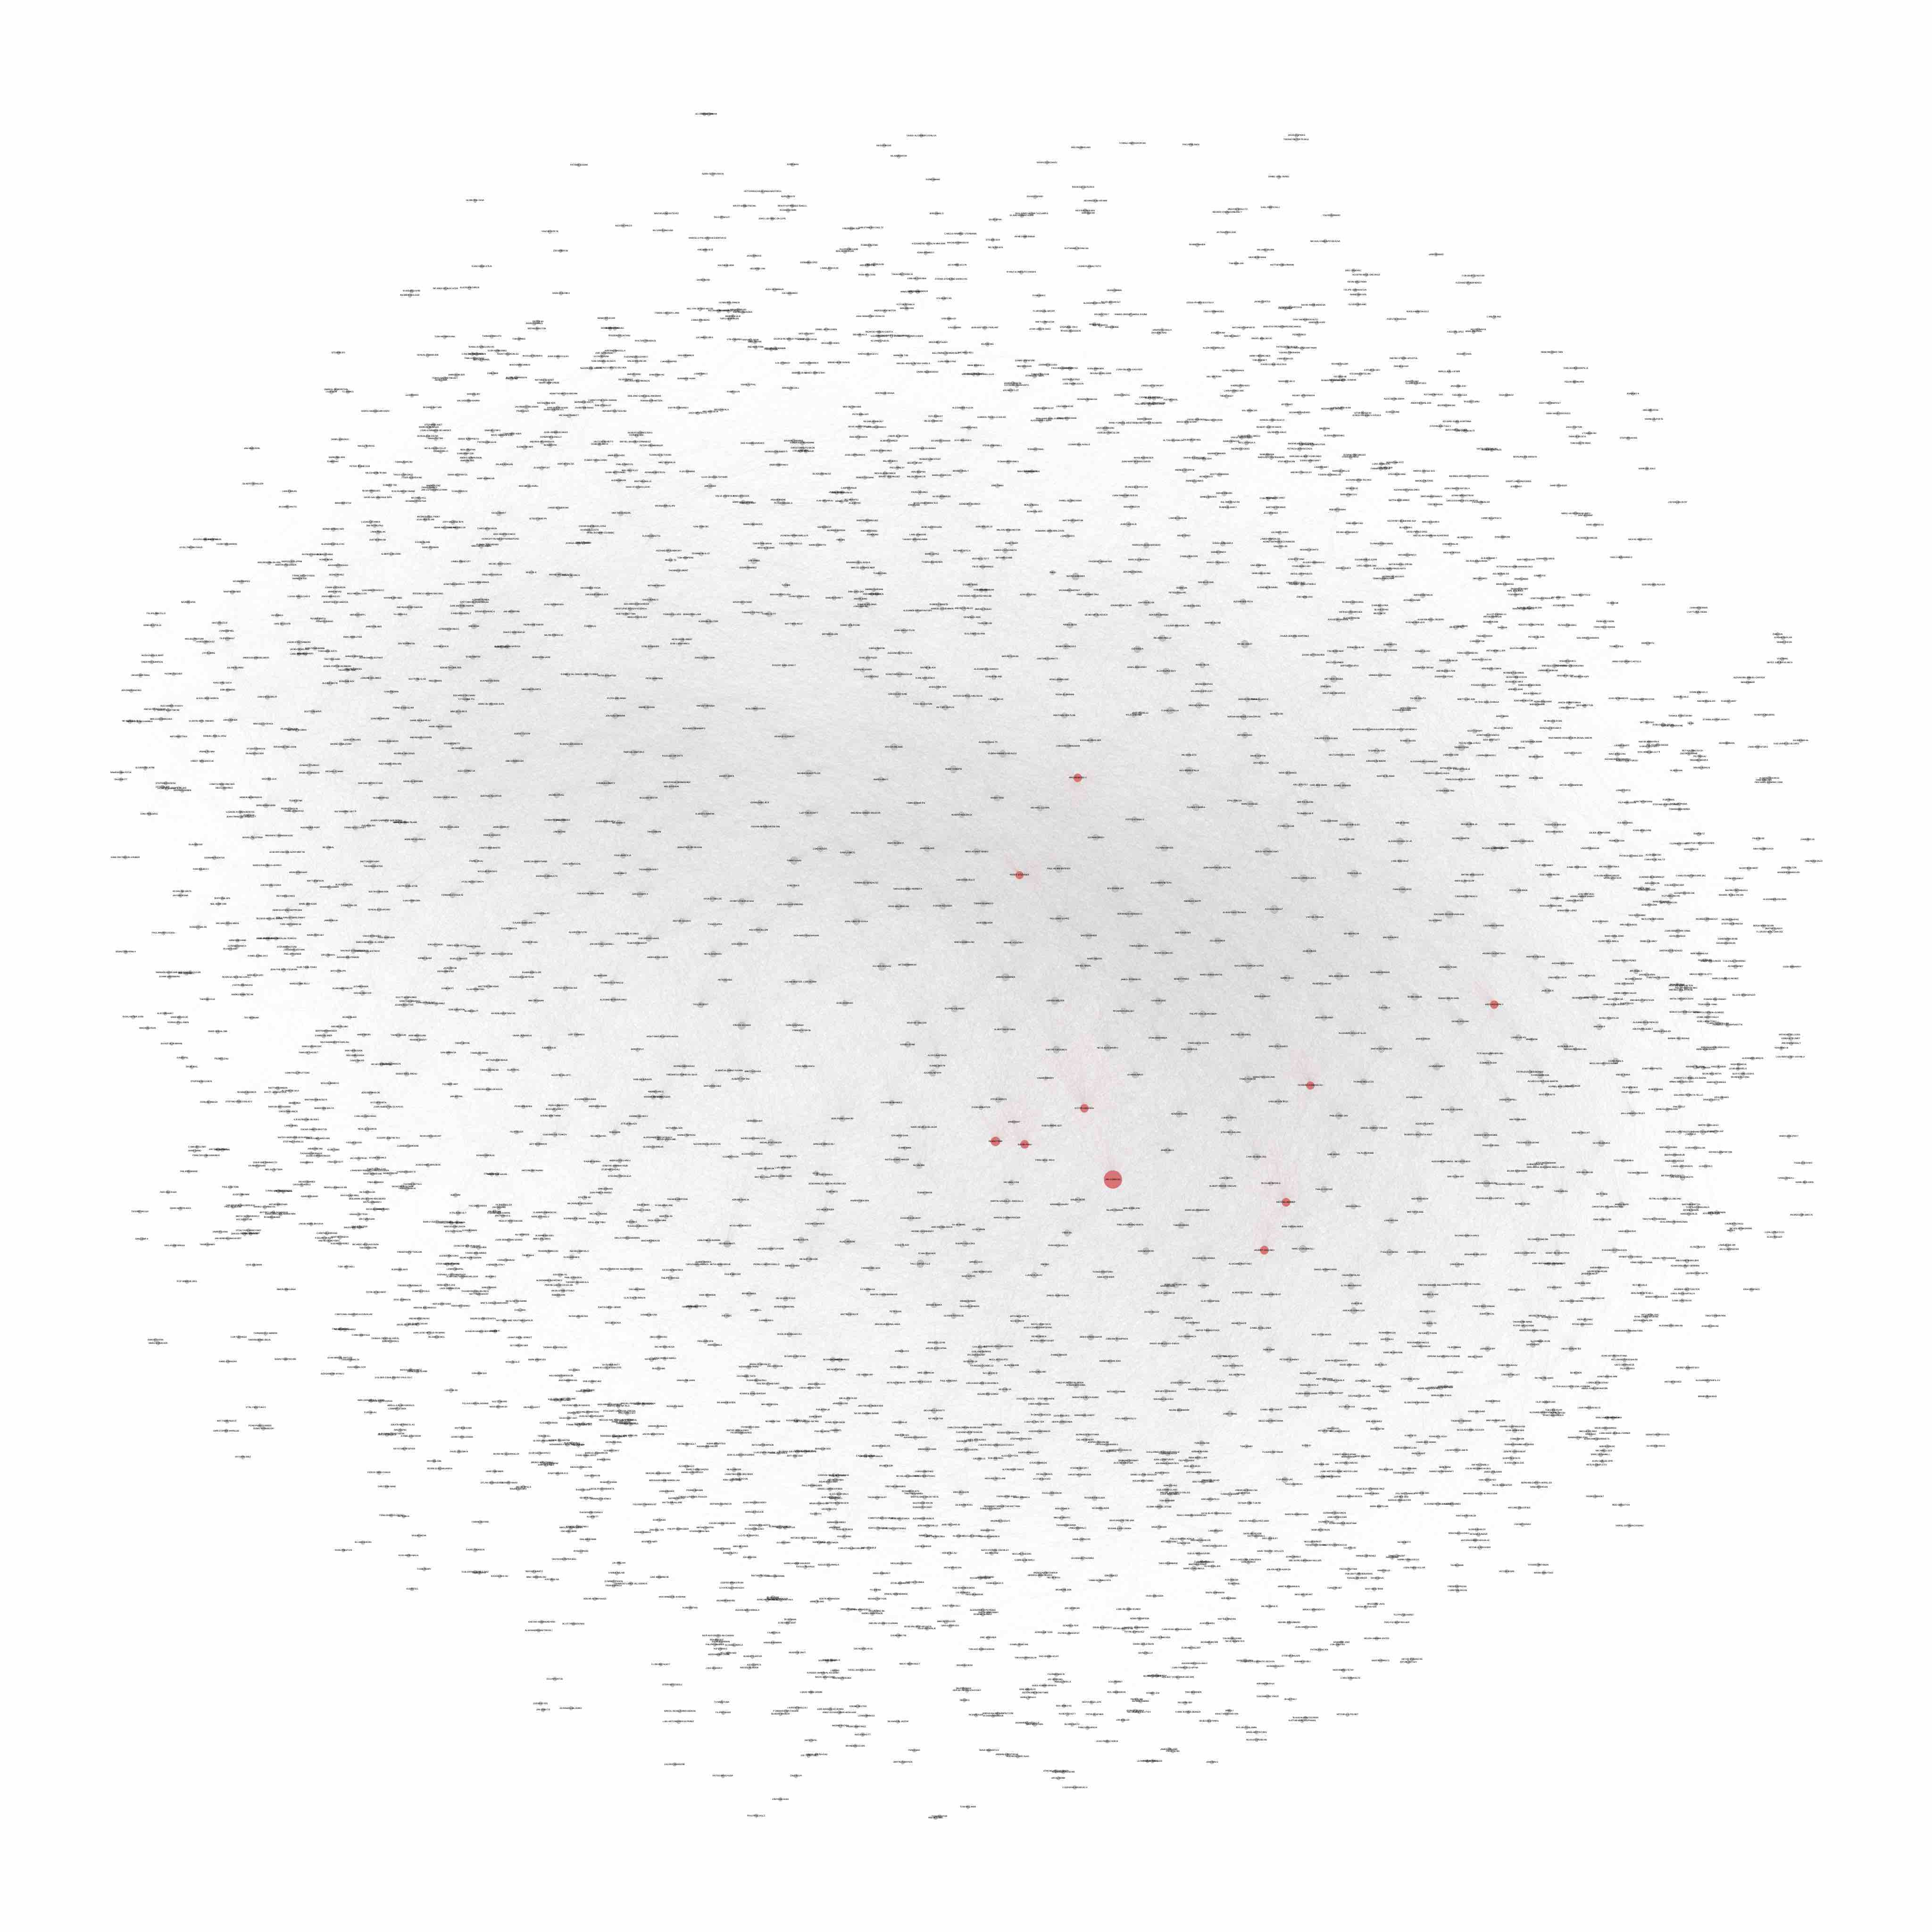
\includegraphics[width=\textwidth]{3a_harmonic_centrality}
\caption{Harmonic Centrality in network} \label{fig_3a_harmonic_centrality}
\end{figure}

\begin{table}
\centering
\caption{Degree vs Eigen}\label{tab_degree_eigen}
\begin{tabular}{|l|l|l|l|l|}
\hline
\# & Degree & value & Eigen & value \\ \hline
1 & TOMMY-HAAS & 0.106 & ROGER-FEDERER & 0.234 \\ \hline
2 & ROGER-FEDERER & 0.1 & RAFAEL-NADAL & 0.192 \\ \hline
3 & MIKHAIL-YOUZHNY & 0.098 & NOVAK-DJOKOVIC & 0.188 \\ \hline
4 & RAINER-SCHUETTLER & 0.098 & DAVID-FERRER & 0.173 \\ \hline
5 & JARKKO-NIEMINEN & 0.098 & ANDY-MURRAY & 0.156 \\ \hline
6 & LLEYTON-HEWITT & 0.098 & TOMAS-BERDYCH & 0.153 \\ \hline
7 & FELICIANO-LOPEZ & 0.097 & MIKHAIL-YOUZHNY & 0.132 \\ \hline
8 & TOMMY-ROBREDO & 0.097 & ANDY-RODDICK & 0.13 \\ \hline
9 & RADEK-STEPANEK & 0.095 & FERNANDO-VERDASCO & 0.128 \\ \hline
10 & CARLOS-MOYA & 0.095 & TOMMY-ROBREDO & 0.128 \\ \hline

\end{tabular}
\end{table}

	The top 10 Degree and Eigen centrality is shown in Table.~\ref{tab_degree_eigen}. Both centralities agrees with each other. Moreover, the top 10 Eigen centrality is the same as Katz centrality. With Table .~\ref{tab_eigen_real}, we can see that Katz centrality is almost aligned with real performance of players in terms of ranking of grand slam (GS) title, tournament titles and GOAT points. In some way, we can conclude that the number of matches fought by a player reflects the players quantity and competitiveness. For example, in a grand slam tournament with 128 players, the champion has to win 7 consecutive matches. A player who wants to win must play more matches than others. With that being said, the high correlation with degree and Katz centrality is understandable. Looking into Fig.~\ref{fig_3a_degree_centrality} and Fig.~\ref{fig_3a_eigen_centrality}, we can clearly sees that the top 10 plays are more center inside "competitive" oval.

\begin{table}
\centering
\caption{Eigen Centrality vs Reality} \label{tab_eigen_real}
\begin{tabular}{|l|l|l|l|l|l|l|}
\hline

\# & Name & Won & Won & GOAT* & Active & Highest Ranking \\ 
 &  & GS & Title & point & Year & (achieved date) \\ \hline
1 & Roger Federer & 20 & 103 & 201 & 1998- & 1(2004.02) \\ 
2 & Rafael Nadal & 19 & 84 & 168 & 2001- & 1(2008.08) \\ 
3 & Novak Djokovic & 16 & 77 & 185 & 2003- & 1(2011.07) \\ 
4 & David Ferrer & 0 & 27 & 124 & 2000-2019 & 3(2013.07) \\ 
5 & Andy Murray & 3 & 46 & 57 & 2005- & 1(2016.11) \\ 
6 & Tomas Berdych & 0 & 13 & 32 & 2002-2019 & 4(2015.05) \\ 
7 & Mikhail Youzhny & 0 & 10 & 27 & 1999-2019 & 8(2008.01) \\ 
8 & Andy Roddick & 1 & 32 & 33 & 2000-2012 & 1(2003.11) \\ 
9 & Tommy Robredo & 0 & 12 & 32 & 1998- & 5(2006.08) \\ 
10 & Fernando Verdasco & 0 & 7 & 22 & 2001- & 7(2009.04) \\ \hline

\end{tabular}
\end{table}


\begin{figure}
\centering
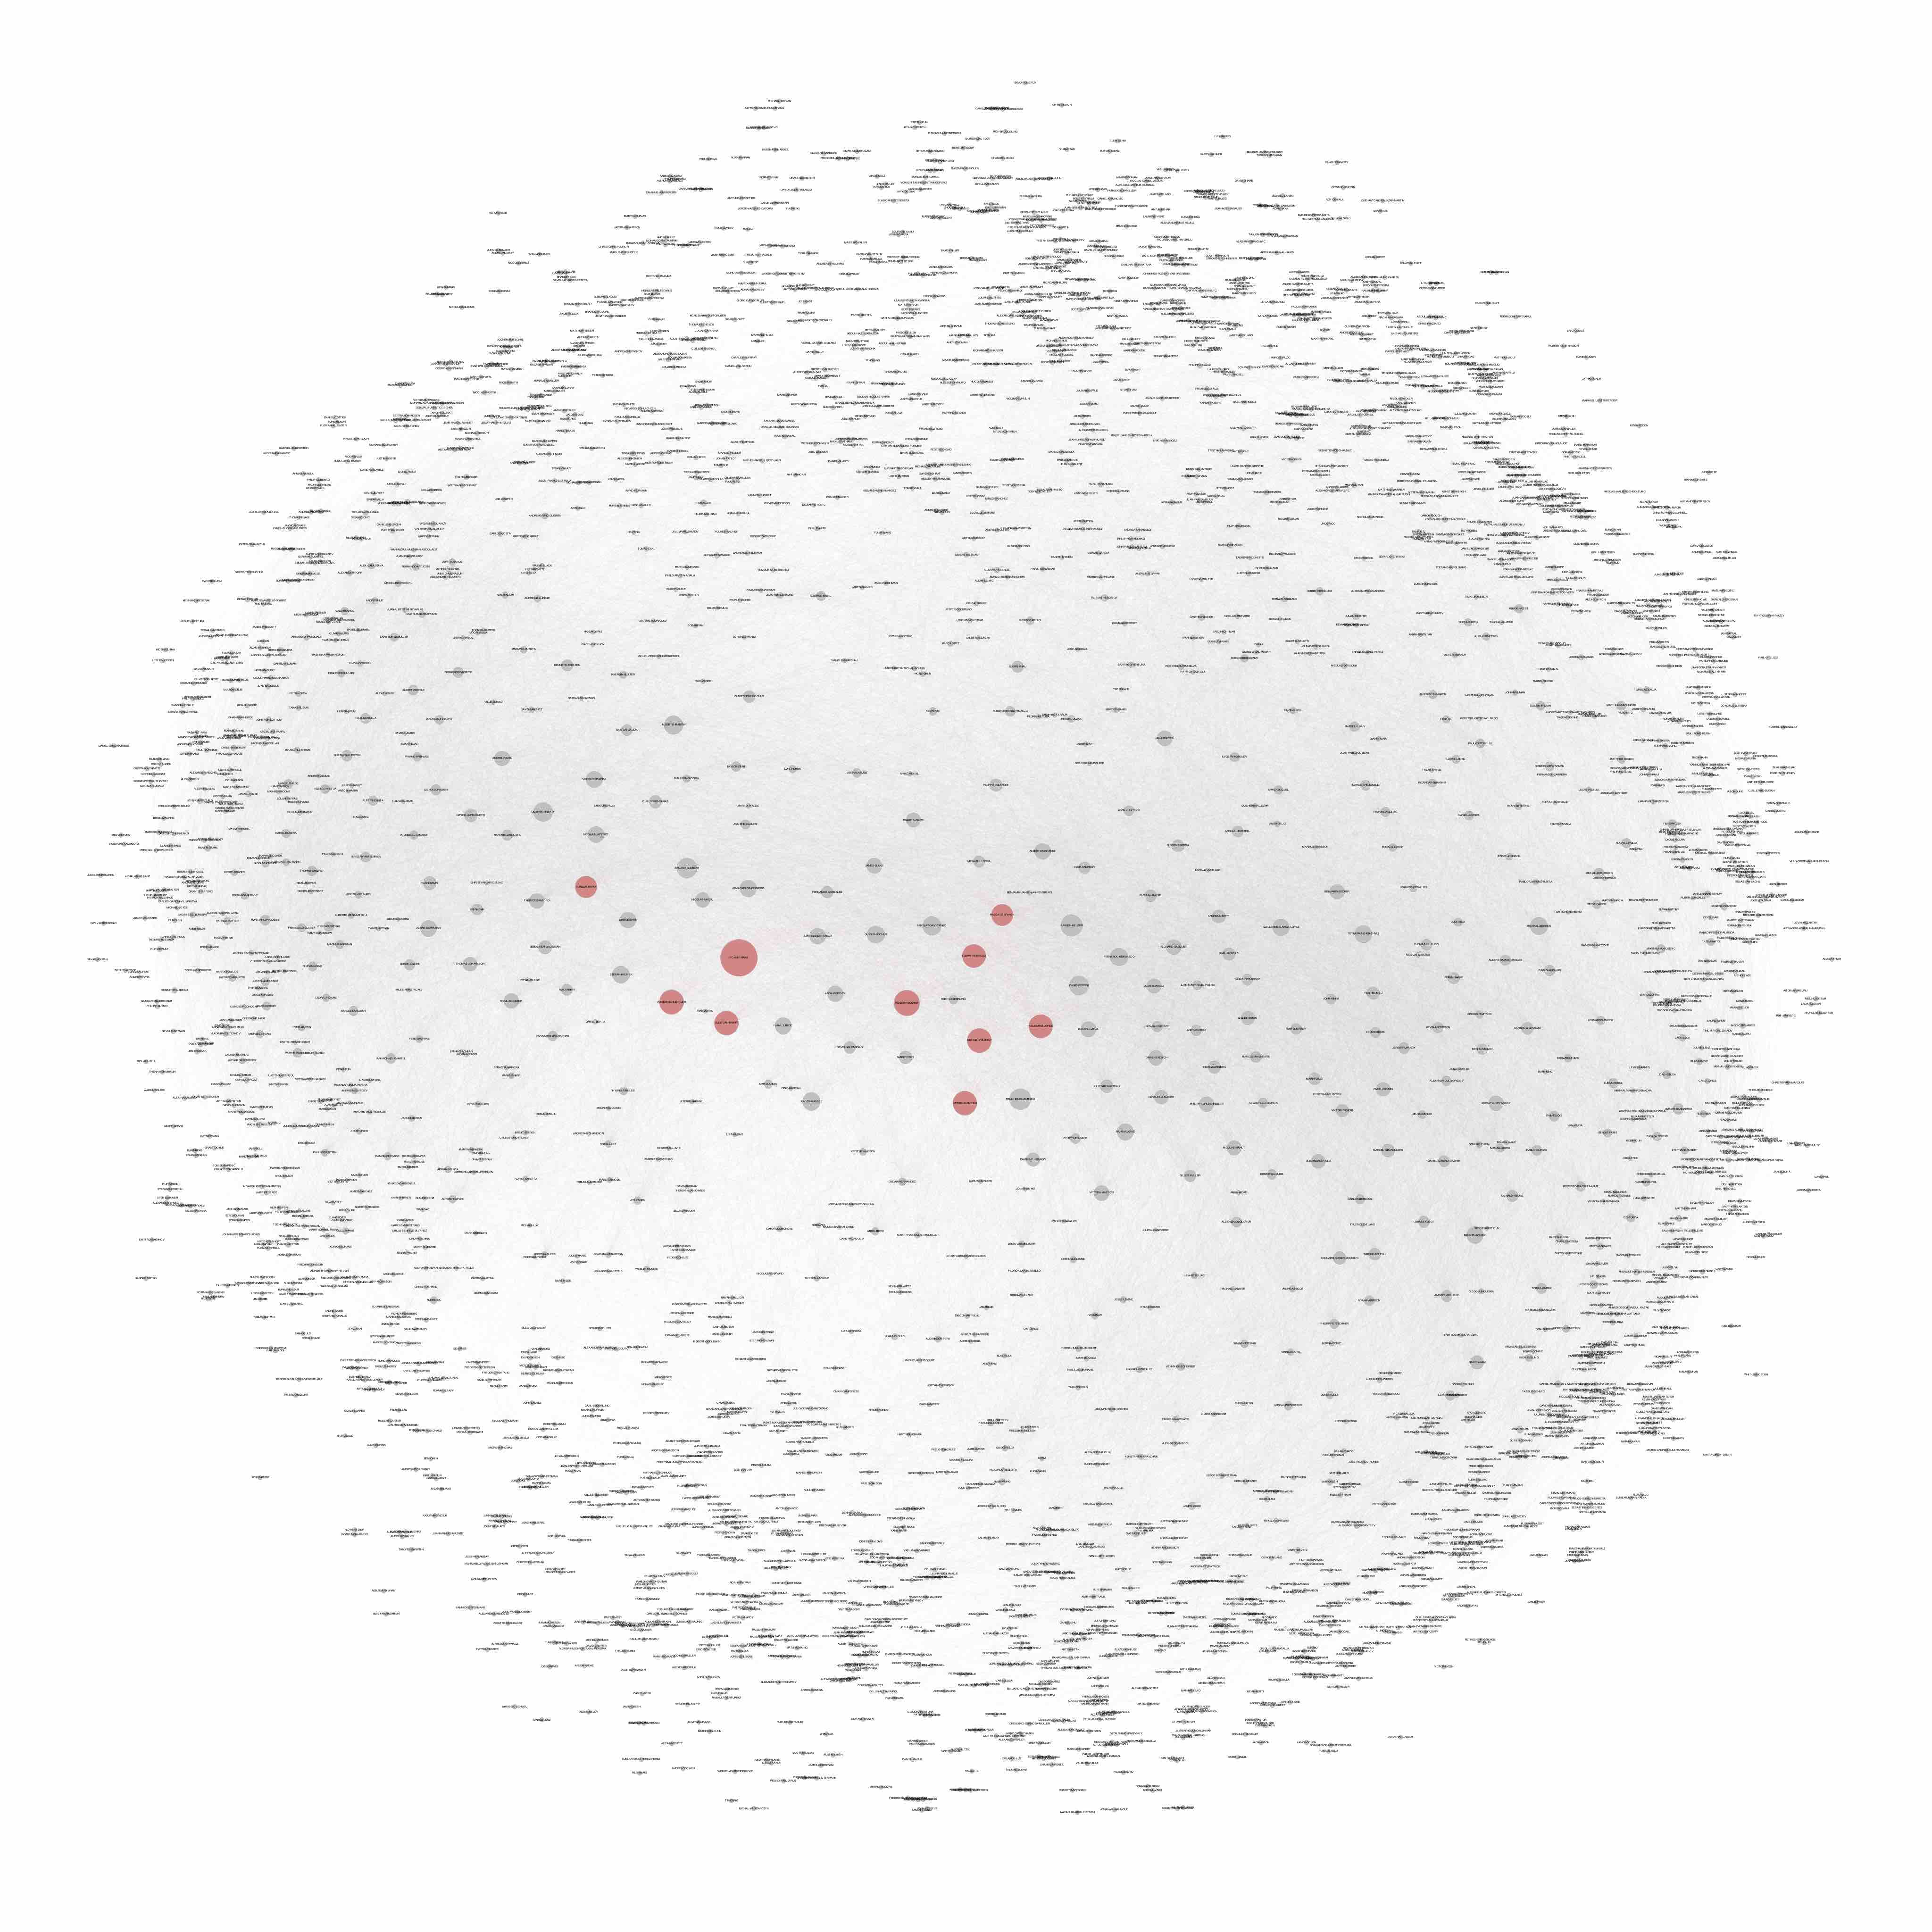
\includegraphics[width=\textwidth]{3a_degree_centrality}
\caption{Degree Centrality} \label{fig_3a_degree_centrality}
\end{figure}


\begin{figure}
\centering
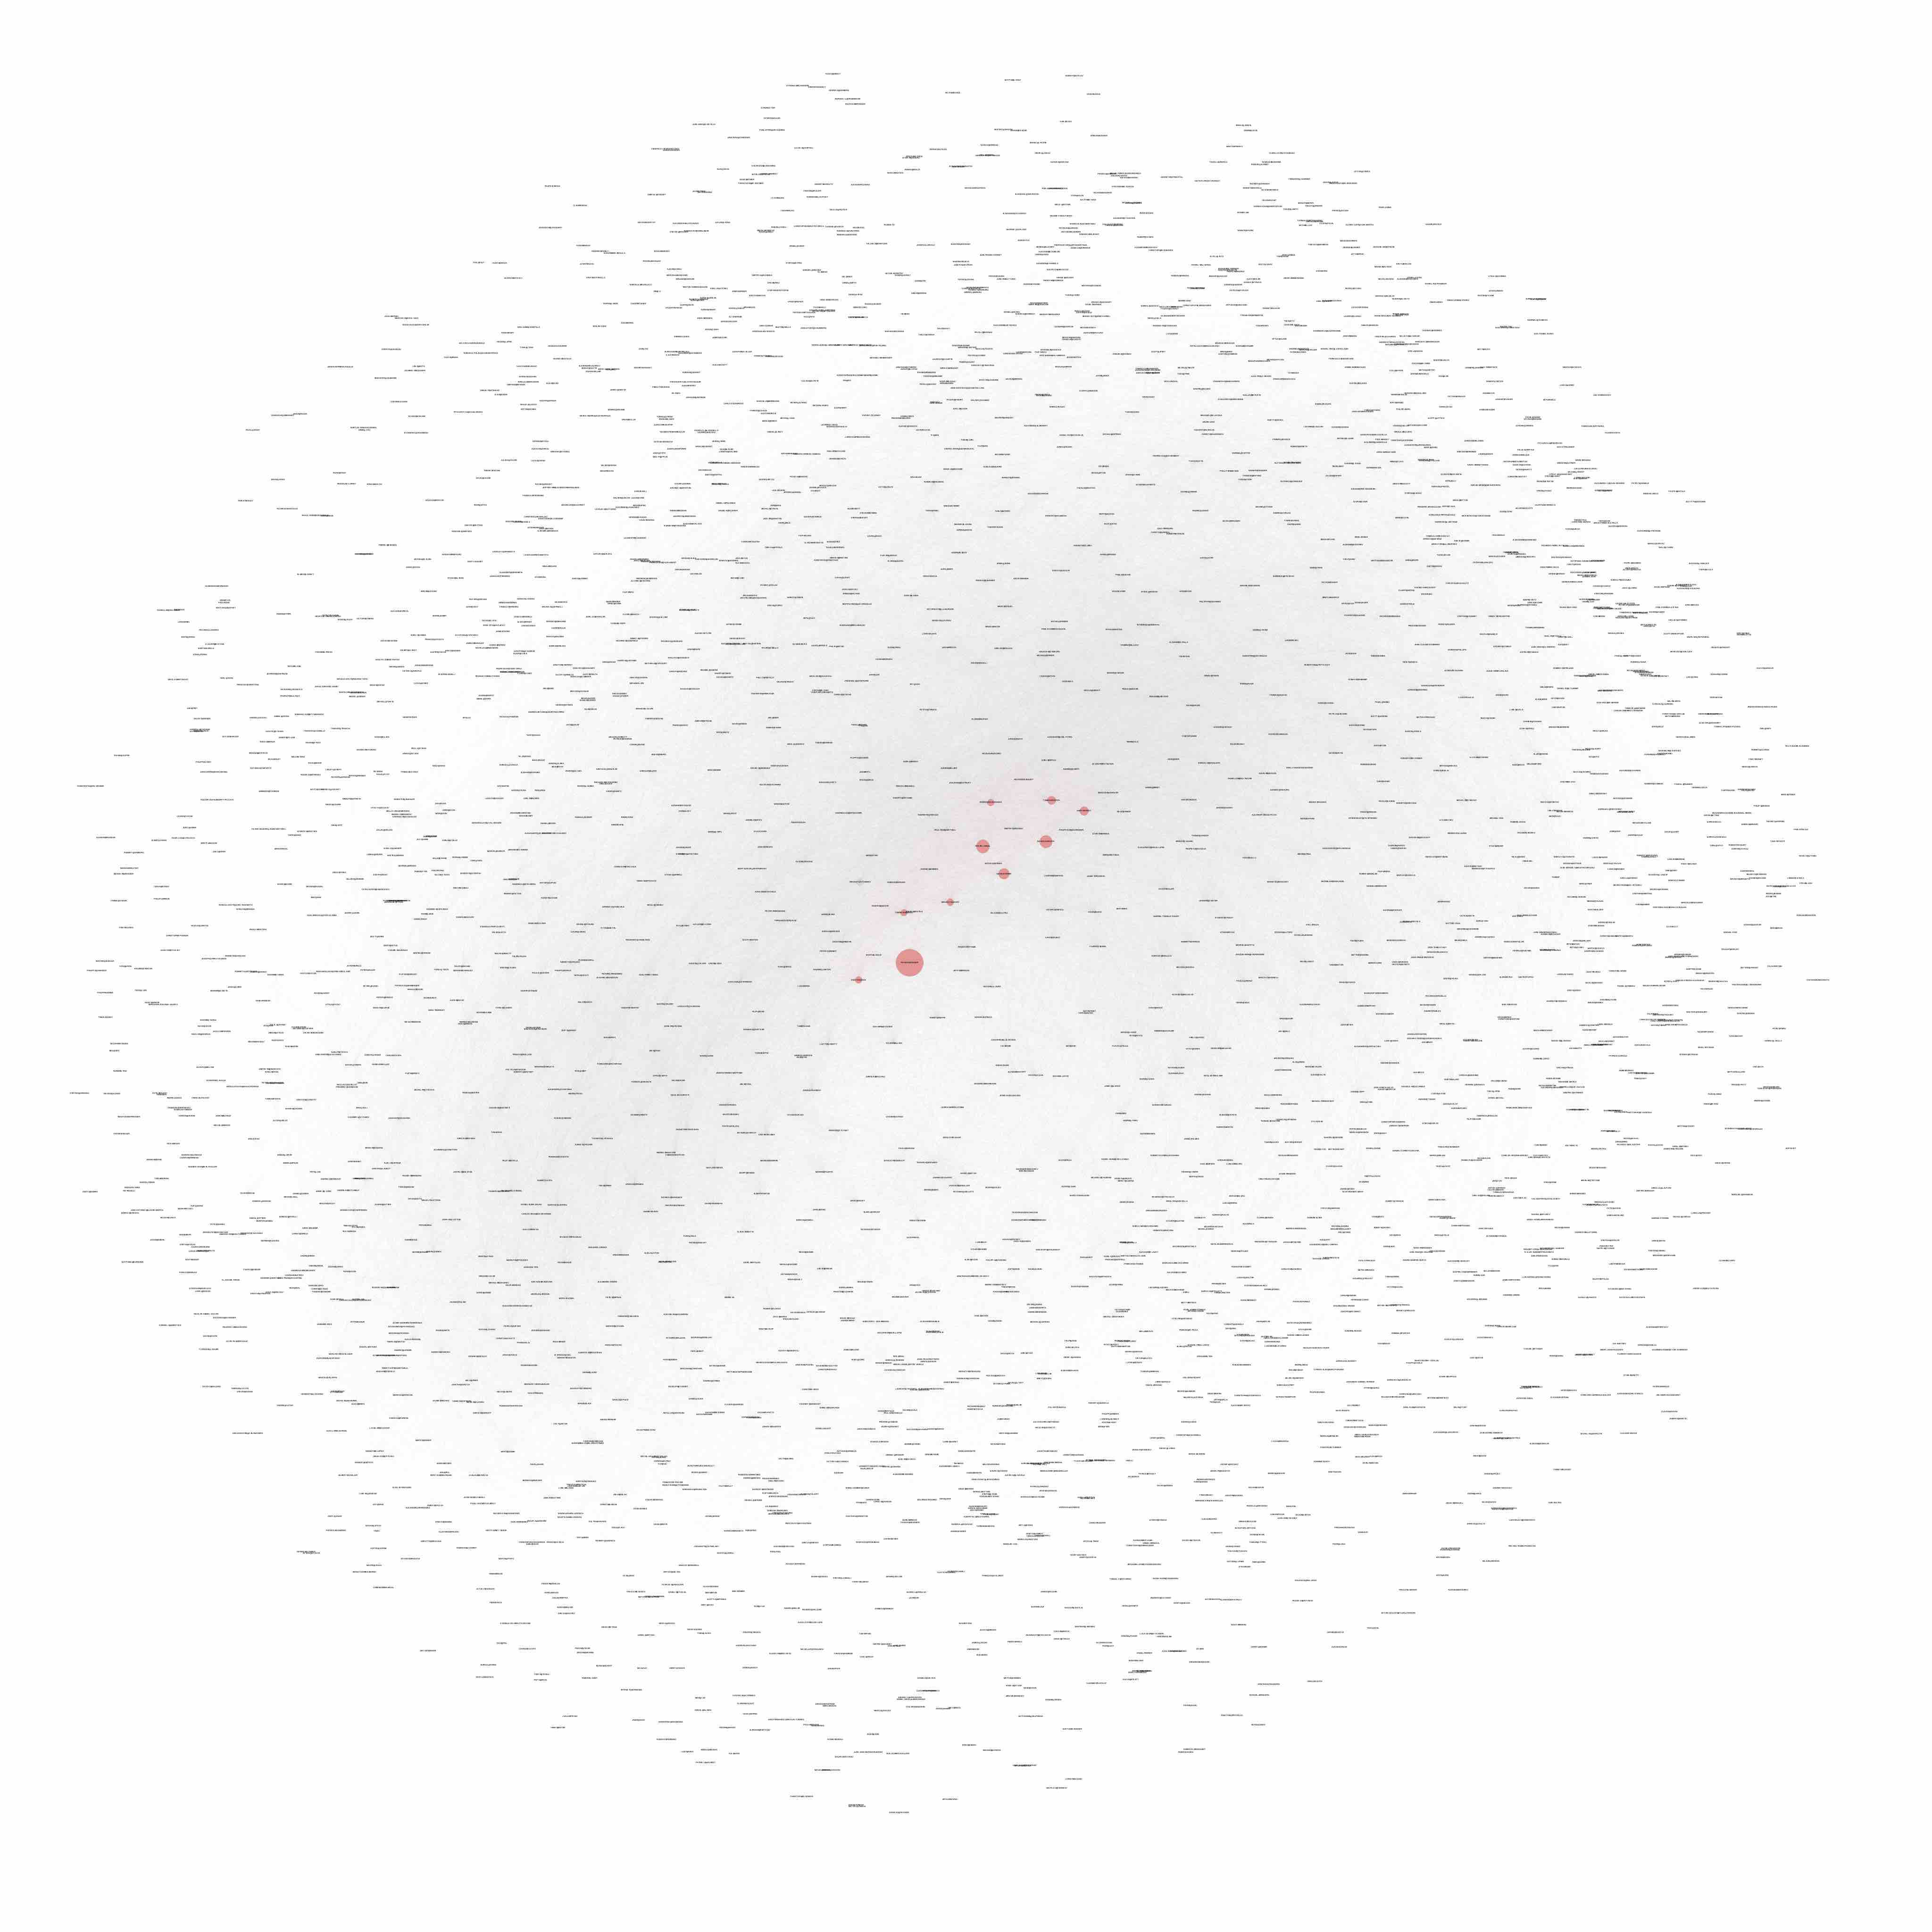
\includegraphics[width=\textwidth]{3a_eigen_centrality}
\caption{Eigen Centrality} \label{fig_3a_eigen_centrality}
\end{figure}

Fig.~\ref{fig_3a_degreebet_centralityplot} and Fig.~\ref{fig_3a_degree_harmonic_centralityplot} shows the scatter plot between betweenness and degree centrality and the one between harmonic and degree centrality. For the between betweenness and degree centrality, we cannot identify a direct correlation for two parameters. For the correlation between harmonic and degree centrality, , the harmonic centrality grows significantly from average degree 0 to 0.02. After that, the growing in harmonic saturates. Although one can say that harmonic is linear to degree, the variation from nodes and almost ceiling value make correlation unrealistic.


\begin{figure}
    \centering
    \begin{minipage}{0.5\textwidth}
        \centering
        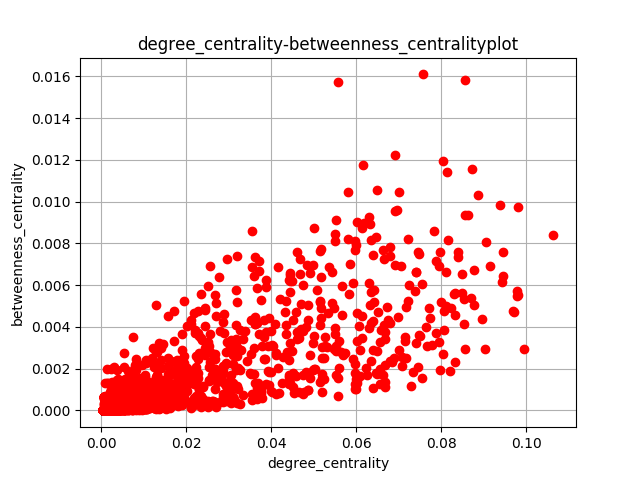
\includegraphics[width=\textwidth]{3a_degree_centrality-betweenness_centralityplot} % first figure itself
        \caption{\(B_{i}\) vs. \(k_{i}\)}
        \label{fig_3a_degreebet_centralityplot}
    \end{minipage}\hfill
    \begin{minipage}{0.5\textwidth}
        \centering
        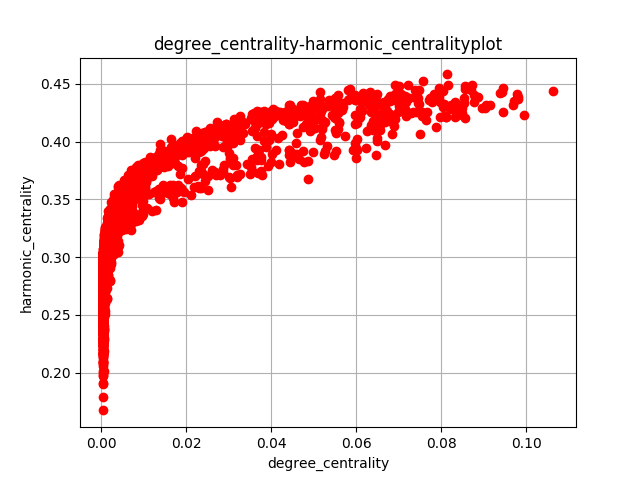
\includegraphics[width=\textwidth]{3a_degree_centrality-harmonic_centralityplot} % second figure itself
        \caption{\(H*_{i}\)  vs.  \(k_{i}\)}
        \label{fig_3a_degree_harmonic_centralityplot}
    \end{minipage}
\end{figure}

One the other hand, Fig.~\ref{fig_3a_plot_eigen}  shows that Eigen centrality is close to a exponential function of degree centrality. The correlation of two centrality is evident. However, as the of degree nodes grow higher, the nodes becomes more separated. Using degree centrality as an index for evaluating student is far from ideal. 

\begin{figure}
\centering
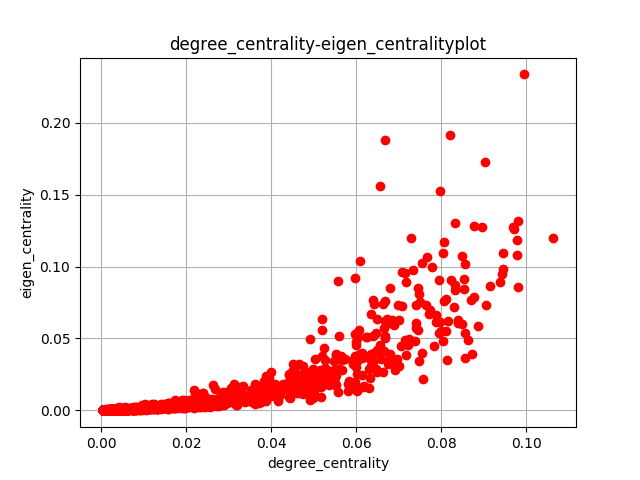
\includegraphics[width=\textwidth]{3a_degree_eigen_plot}
\caption{ \(E_{i}\) vs. \(k_{i}\)} 
\label {fig_3a_plot_eigen}
\end{figure}


For Katz centrality, I have choose \(\alpha = 0.9*\frac{1}{\lambda} \) to guarantee the convergence of Katz computation. I have computed rank for 4 different \(\beta\) value, 0.1, 0.2, 0.5 and 1. It turns out that the both the ranks and values to 3 decimal point remain the same regardless of different \(\beta\). \(\beta\) has no influence on top ranked Katz centrality. Moreover, the rank is identical to that of Eigen centrality. This can be understood by the fact that Katz centrality is an adaptation of Eigen centrality with adjustment constant \(\alpha \) and \(\beta\). By comparing the top 10 ranking of Katz centrality to real world statistics of player, we can see that they agree with each other.


\begin{table}
\centering
\caption{Katz Centrality vs Reality} \label{tab_katz_real}
\begin{tabular}{|l|l|l|l|l|l|l|}
\hline

\# & Name & Won & Won & GOAT* & Active & Highest Ranking \\ 
 &  & GS & Title & point & Year & (achieved date) \\ \hline
1 & Roger Federer & 20 & 103 & 201 & 1998- & 1(2004.02) \\ 
2 & Rafael Nadal & 19 & 84 & 168 & 2001- & 1(2008.08) \\ 
3 & Novak Djokovic & 16 & 77 & 185 & 2003- & 1(2011.07) \\ 
4 & David Ferrer & 0 & 27 & 124 & 2000-2019 & 3(2013.07) \\ 
5 & Andy Murray & 3 & 46 & 57 & 2005- & 1(2016.11) \\ 
6 & Tomas Berdych & 0 & 13 & 32 & 2002-2019 & 4(2015.05) \\ 
7 & Mikhail Youzhny & 0 & 10 & 27 & 1999-2019 & 8(2008.01) \\ 
8 & Andy Roddick & 1 & 32 & 33 & 2000-2012 & 1(2003.11) \\ 
9 & Tommy Robredo & 0 & 12 & 32 & 1998- & 5(2006.08) \\ 
10 & Fernando Verdasco & 0 & 7 & 22 & 2001- & 7(2009.04) \\ \hline

\end{tabular}
\end{table}

For Katz centrality, I have choose \(\alpha = 0.85\) for striking a balance with random jump probability. Table~\ref{tab_katz_vs_page} is shown with the comparison with Katz centrality. Among the top 10 players, 2 players are the of the same rank, 6 players are presence in both rank, 2 players are different. Looking into the top 11~20 of page rank, players who are presence in top 10 in Katz appear.
For example, Andy Roddick is 17th ranked and Andy Murray 14th in page rank. The values of their centrality is very close to each other, only by 0.001
The reality compassion of page rank is shown in Table~\ref{tab_page_real}. It is obvious that page rank disagree greatly in the order of rank of reality. For example, in page rank, David Ferrer is ranked 2nd, 2 place higher in Katz while Novak Djokovic is ranked 6th, 3 place lower. 
Still, page rank is strongly correlated with Katz centrality to a degree that is almost linear. Fig.\ref{fig_3a_page_katz_plot} shown the scatter plot between the two. The variation appears around page rank larger 0.002. In the higher ranked region, the disagreement is visually identifiable. The reason that Page Rank is not suitable for evaluating a player is due to part of the nature of page rank. Page Rank is originally designed for web pages with the assumption that a web page is more relevant than
another if it is pointed by another important page. This is almost the case with Katz. However, the introduction of the "random jump" makes non-sense in the player network. That explains the variation in ranking of page rank compared with Katz centrality.

\begin{table}
\centering
\caption{Katz vs Page Rank}\label{tab_katz_vs_page}
\begin{tabular}{|l|l|l|l|l|}
\hline
\# & Katz & value & Page & value \\ \hline
1 & ROGER-FEDERER & 0.199 & ROGER-FEDERER & 0.00536 \\ \hline
2 & RAFAEL-NADAL & 0.162 & DAVID-FERRER & 0.00442 \\ \hline
3 & NOVAK-DJOKOVIC & 0.157 & RAFAEL-NADAL & 0.00417 \\ \hline
4 & DAVID-FERRER & 0.149 & MIKHAIL-YOUZHNY & 0.00396 \\ \hline
5 & ANDY-MURRAY & 0.133 & TOMMY-ROBREDO & 0.00389 \\ \hline
6 & TOMAS-BERDYCH & 0.131 & NOVAK-DJOKOVIC & 0.00381 \\ \hline
7 & MIKHAIL-YOUZHNY & 0.117 & TOMAS-BERDYCH & 0.00379 \\ \hline
8 & ANDY-RODDICK & 0.115 & TOMMY-HAAS & 0.00377 \\ \hline
9 & TOMMY-ROBREDO & 0.114 & FELICIANO-LOPEZ & 0.00375 \\ \hline
10 & FERNANDO-VERDASCO & 0.113 & FERNANDO-VERDASCO & 0.00360 \\ \hline

\end{tabular}
\end{table}


\begin{figure}
\centering
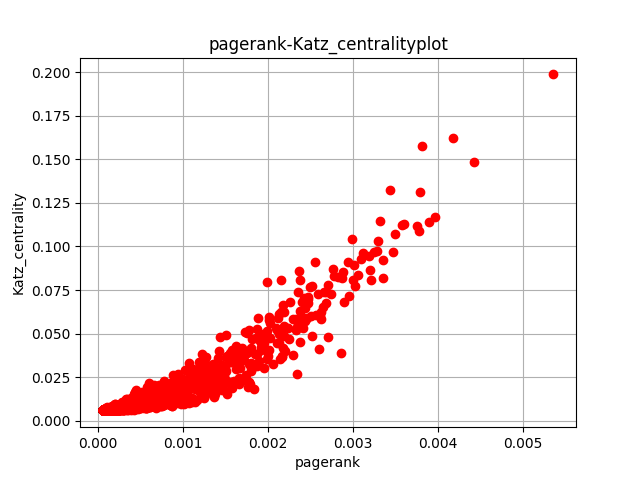
\includegraphics[width=\textwidth]{3b_pagerank-Katz_centralityplot}
\caption{Page Rank vs Katz} \label{fig_3a_page_katz_plot}
\end{figure}

\begin{table}
\centering
\caption{Page Rank vs Reality}\label{tab_page_real}
\begin{tabular}{|l|l|l|l|l|l|l|}
\hline

\# & Name & Won & Won & GOAT* & Active & Highest Ranking \\ 
 &  & GS & Title & point & Year & (achieved date) \\ \hline
1 & Roger Federer & 20 & 103 & 201 & 1998- & 1(2004.02) \\ 
2 & David Ferrer & 0 & 27 & 124 & 2000-2019 & 3(2013.07) \\ 
3 & Rafael Nadal & 19 & 84 & 168 & 2001- & 1(2008.08) \\ 
4 & Mikhail Youzhny & 0 & 10 & 27 & 1999-2019 & 8(2008.01) \\ 
5 & Tommy Robredo & 0 & 12 & 32 & 1998- & 5(2006.08) \\ 
6 & Novak Djokovic & 16 & 77 & 185 & 2003- & 1(2011.07) \\ 
7 & Tomas Berdych & 0 & 13 & 32 & 2002-2019 & 4(2015.05) \\ 
8 & Tommy Haas & 0 & 15 & 58 & 1996-2017 & 2(2002.05) \\ 
9 & Feliciano Lopez & 0 & 7 & 22 & 1997- & 12(2015.03) \\ 
10 & Fernando Verdasco & 0 & 7 & 22 & 2001- & 7(2009.04) \\ \hline

\end{tabular}
\end{table}


The result of centrality comparison has fulfilled my motivation of this project. Harmonic and Betweenness Centrality is totally uncorrelated to evaluation player. Although Page Rank ranking is very similar to Katz and Eigen centrality, the top ranked players is somewhat misaligned. Degree and Eigen Centrality is highly correlated to the evaluation player, almost aligned with GS, title and ATP ranking. For Eigen and Katz centrality, a node is important if it is the neighbor of other important node. This is the same case of player ranking, since the quality of a player is reflected by his opponent. Given that Katz centrality is an adoption of Eigen with adjustable weighting parameter \(\alpha \) and \(\beta\). Therefore, I would conclude that  Katz centrality is suitable for evaluation of player in a player network.

% Section of Network Model
\section{Network Model}

In this section, I will be discussing network model. By comparing with random network, small world  and preferential attachment. All the network models are constructed using NetworkX's native function.

For random network, I used Erdős-Rényi model to construct. I set the node size \(N = 3035\) and probability \( \frac{<k>}{N-1} =0.015 \). The \( <k> \) is the average degree of my network, which is 49.075. Table~\ref{tab_random} lists the structural metric for my random graph.

\begin{table}
\centering
\caption{Structural Metrics of Random Network.}\label{tab_random}
\begin{tabular}{|l|l|}
\hline
metric & value \\
\hline
average degree & 49.154 \\
order & 3035 \\
size & 74591 \\
density & 0.016201 \\
diameter & 3 \\
radius & 3 \\
average path length & 2.427481 \\
average clustering coefficient & 0.016153 \\
transitivity & 0.016151 \\
number of triangle & 19729 \\
number of clique & 53269 \\
number of component & 1 \\
\hline
\end{tabular}
\end{table}

Both the average path length and clustering coefficient are lower than that of original network. There is only one component. No disconnected node appears. I calculated the critical value for deciding which region the random graph lands. With \(<k> = 49.152 > ln(N) = ln(3035) = 8\), the random graph is Supercritical with one giant component. Moreover, the clustering coefficient is shown in Fig.~\ref{fig_4a_clustering_coeff} and  Fig.~\ref{fig_4a_clustering_coeff_log}. With random graph, the clustering coefficient is almost identical for every node regardless of degree. The degree distribution is show in Fig.~\ref{fig_4a_degreedist_hist} and  Fig.~\ref{fig_4a_degreedist_log}. The result is close to a poisson distribution with \( \lambda = 49 \). Fig.~\ref{fig_4a_random_graph} shows the network of random graph. In the figure, there are no visible big hubs. Most of the nodes are of the same order of size, which verifies the degree distribution. 

From the degree and clustering distribution, we can see that the player network is not a random graph. 

\begin{figure}
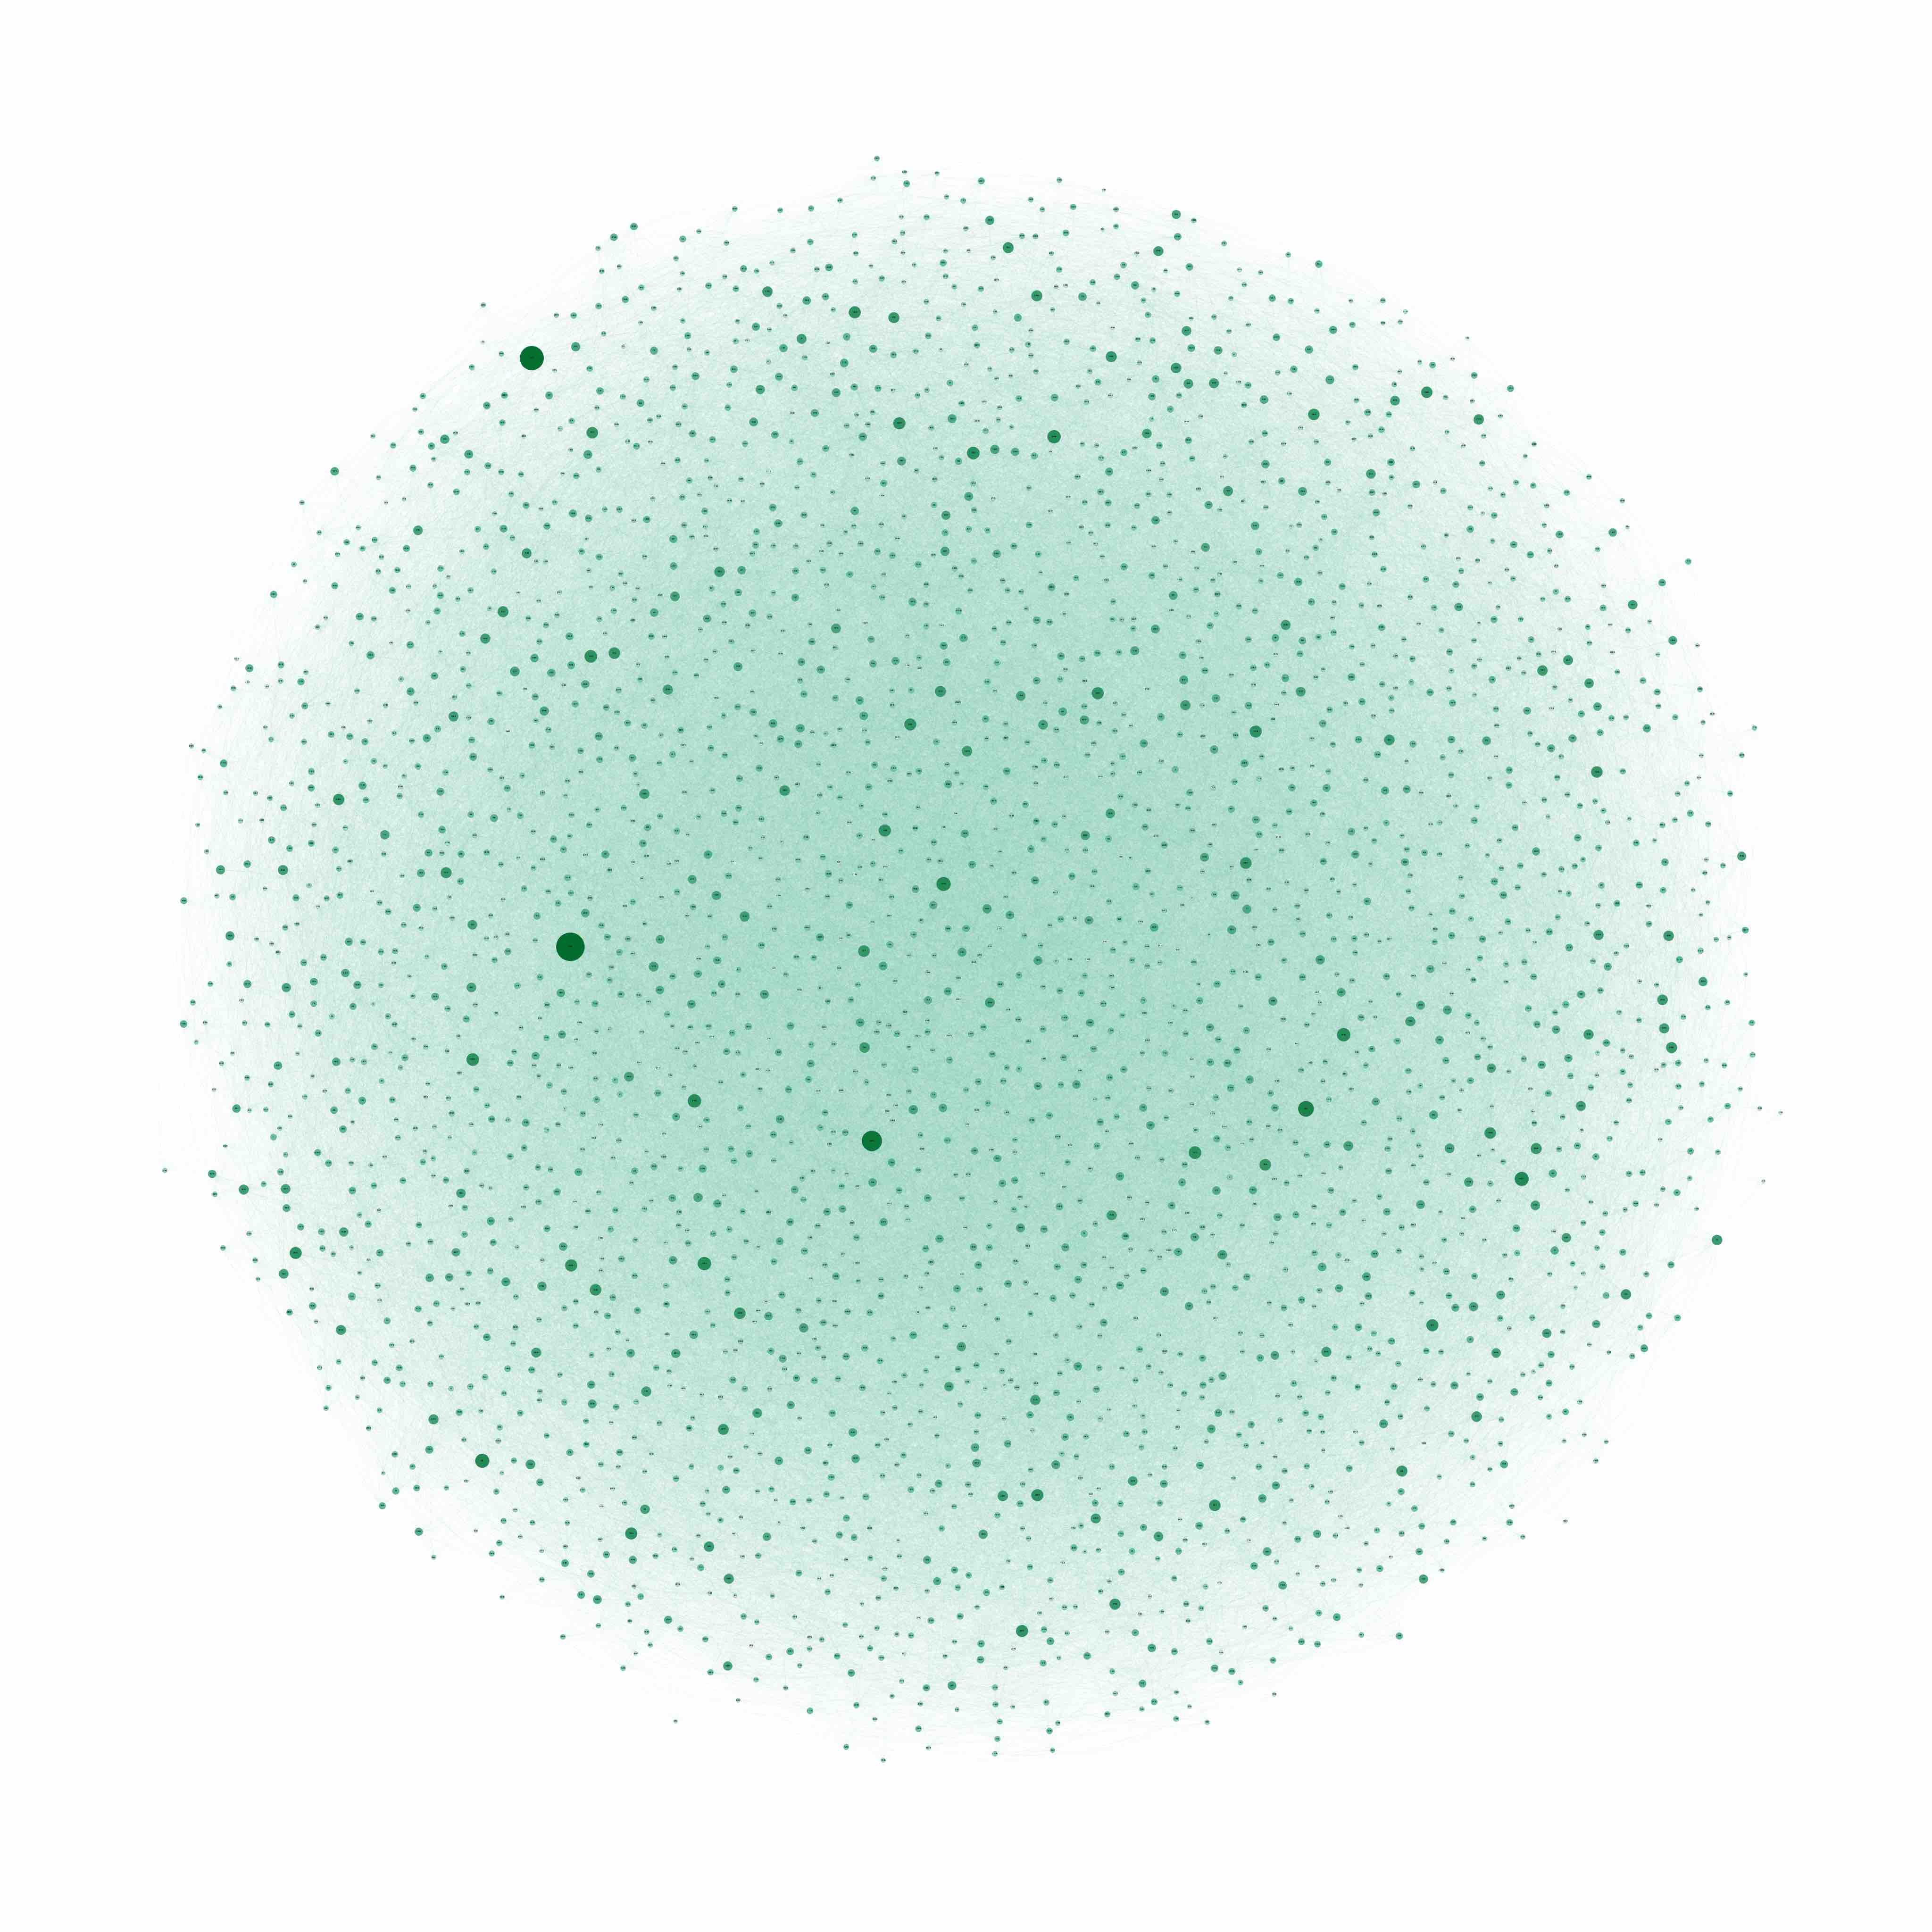
\includegraphics[width=\textwidth]{4a_random_graph}
\caption{Random Network k=3035,p=0.0016} \label{fig_4a_random_graph}
\end{figure}


\begin{figure}
    \centering
    \begin{minipage}{0.5\textwidth}
        \centering
        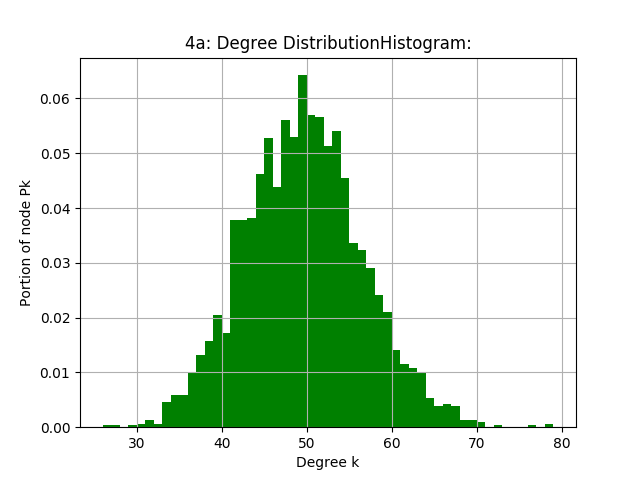
\includegraphics[width=\textwidth]{4a_Degree_dist_hist} % first figure itself
        \caption{Degree Distribution}
        \label{fig_4a_degreedist_hist}
    \end{minipage}\hfill
    \begin{minipage}{0.5\textwidth}
        \centering
        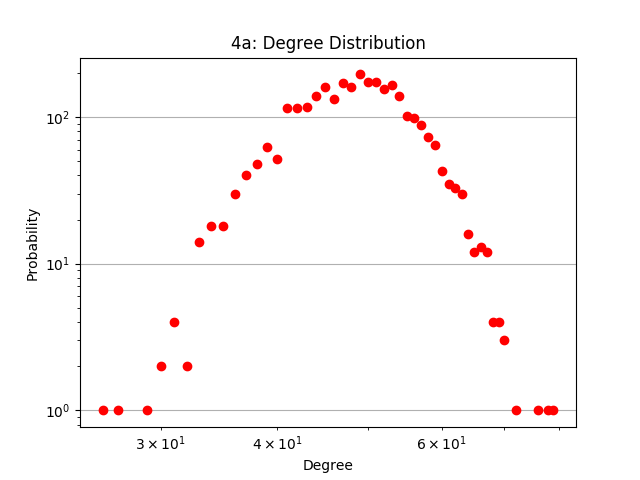
\includegraphics[width=\textwidth]{4a_Degree_dist_log} % second figure itself
        \caption{Degree Distribution in log}
        \label{fig_4a_degreedist_log}
    \end{minipage}
\end{figure}

\begin{figure}
    \centering
    \begin{minipage}{0.5\textwidth}
        \centering
        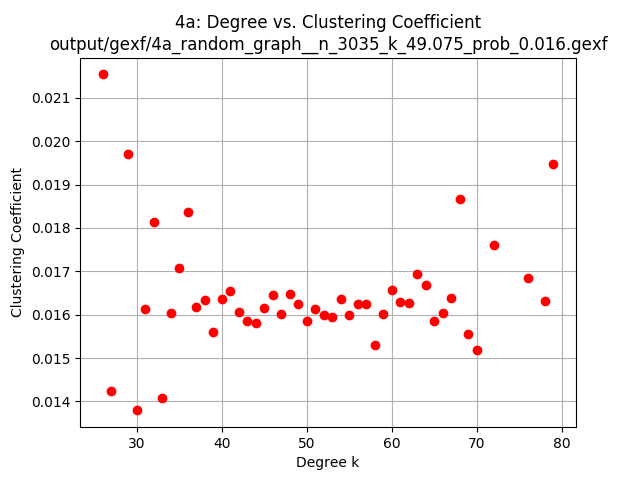
\includegraphics[width=\textwidth]{4a_clustering_coeff} % first figure itself
        \caption{Cluster. Coeff}
        \label{fig_4a_clustering_coeff}
    \end{minipage}\hfill
    \begin{minipage}{0.5\textwidth}
        \centering
        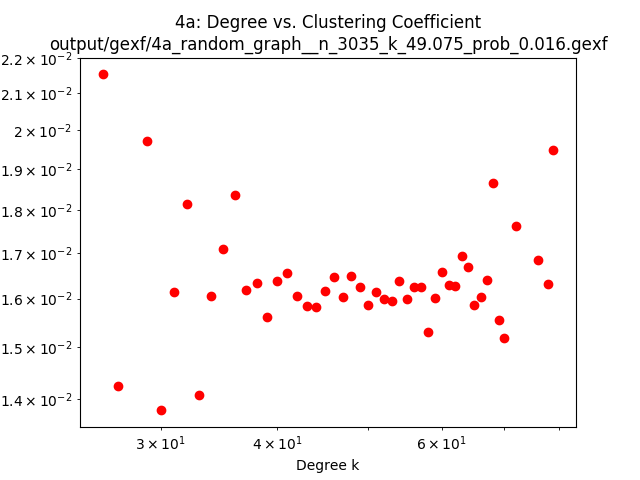
\includegraphics[width=\textwidth]{4a_clustering_coeff_log} % second figure itself
        \caption{Cluster. Coeff in log}
        \label{fig_4a_clustering_coeff_log}
    \end{minipage}
\end{figure}

For small world, I used Watts-Strogatz model to construct. I first generated different small worlds with different probability of rewiring: 0.001, 0.01, 0.05, 0.1, 0.5, 1. Table.~\ref{tab_sm_comparison} shows the smallworldness for each of the generated graph. Therefore, I pick probability of rewiring with 0.05 because this graph has the largest smallworldness, 0.156. I set the node size \(N = 3035\) and number of neighbors for each node \( k =25 \), probability of rewiring \( p = 0.05 \) for my following analysis. The number of neighbors for each node is the half of average degree.

\begin{table}
\centering
\caption{Small Worldness Comparison}\label{tab_sm_comparison}
\begin{tabular}{|l|l|l|l|l|l|l|l|}
\hline
probability & 0.001 & 0.01 & 0.05 & 0.1 & 0.5 & 1 & player network \\ \hline
small worldness & 0.062 & 0.128 & 0.156 & 0.149 & 0.032 & 0.002 & 0.051 \\ \hline
average path length & 11.348 & 5.43 & 3.953 & 3.53 & 2.894 & 2.829 & 3.263 \\ \hline
clustering coefficient & 0.714 & 0.696 & 0.618 & 0.528 & 0.094 & 0.007 & 0.166 \\ \hline

\end{tabular}
\end{table}


\begin{table}
\centering
\caption{Structural Metrics of Small World}\label{tab_smallworld}
\begin{tabular}{|l|l|}
\hline
metric & value \\
\hline
order & 3035 \\
size & 36420 \\
density & 0.007910 \\
diameter & 6 \\
radius & 5 \\
average path length & 3.953023 \\
average clustering coefficient & 0.618777 \\
transitivity & 0.616572 \\
number of triangle & 172503 \\
number of clique & 13260 \\
number of component & 1 \\
\hline
\end{tabular}
\end{table}

Table.~\ref{tab_smallworld} shows the structural metrics of small world. Both the average path length and clustering coefficient are higher than that of original network. This makes sense since small world is started with circular lattice. From the Fig.~\ref{fig_4_smallworld}, we can observe that there remains a structural of lattice. This explains the result of high clustering and average path length. If we choose the rewiring probability to be higher, then the residual circular lattice would become less obvious. The degree distributions are show in Fig.~\ref{fig_4b_sw_degreedist_hist} and  Fig.~\ref{fig_4b_sw_degreedist_log}. The distribution seems to be like a binomial distribution with center in 25. Moreover, the clustering coefficient is shown in Fig.~\ref{fig_4b_sw_clustering_coeff} and  Fig.~\ref{fig_4b_sw_clustering_coeff_log}. With small world, the clustering coefficient is almost identical for every node regardless of degree. From the degree and clustering distribution, we can see that the player network is not a small world. 

\begin{figure}
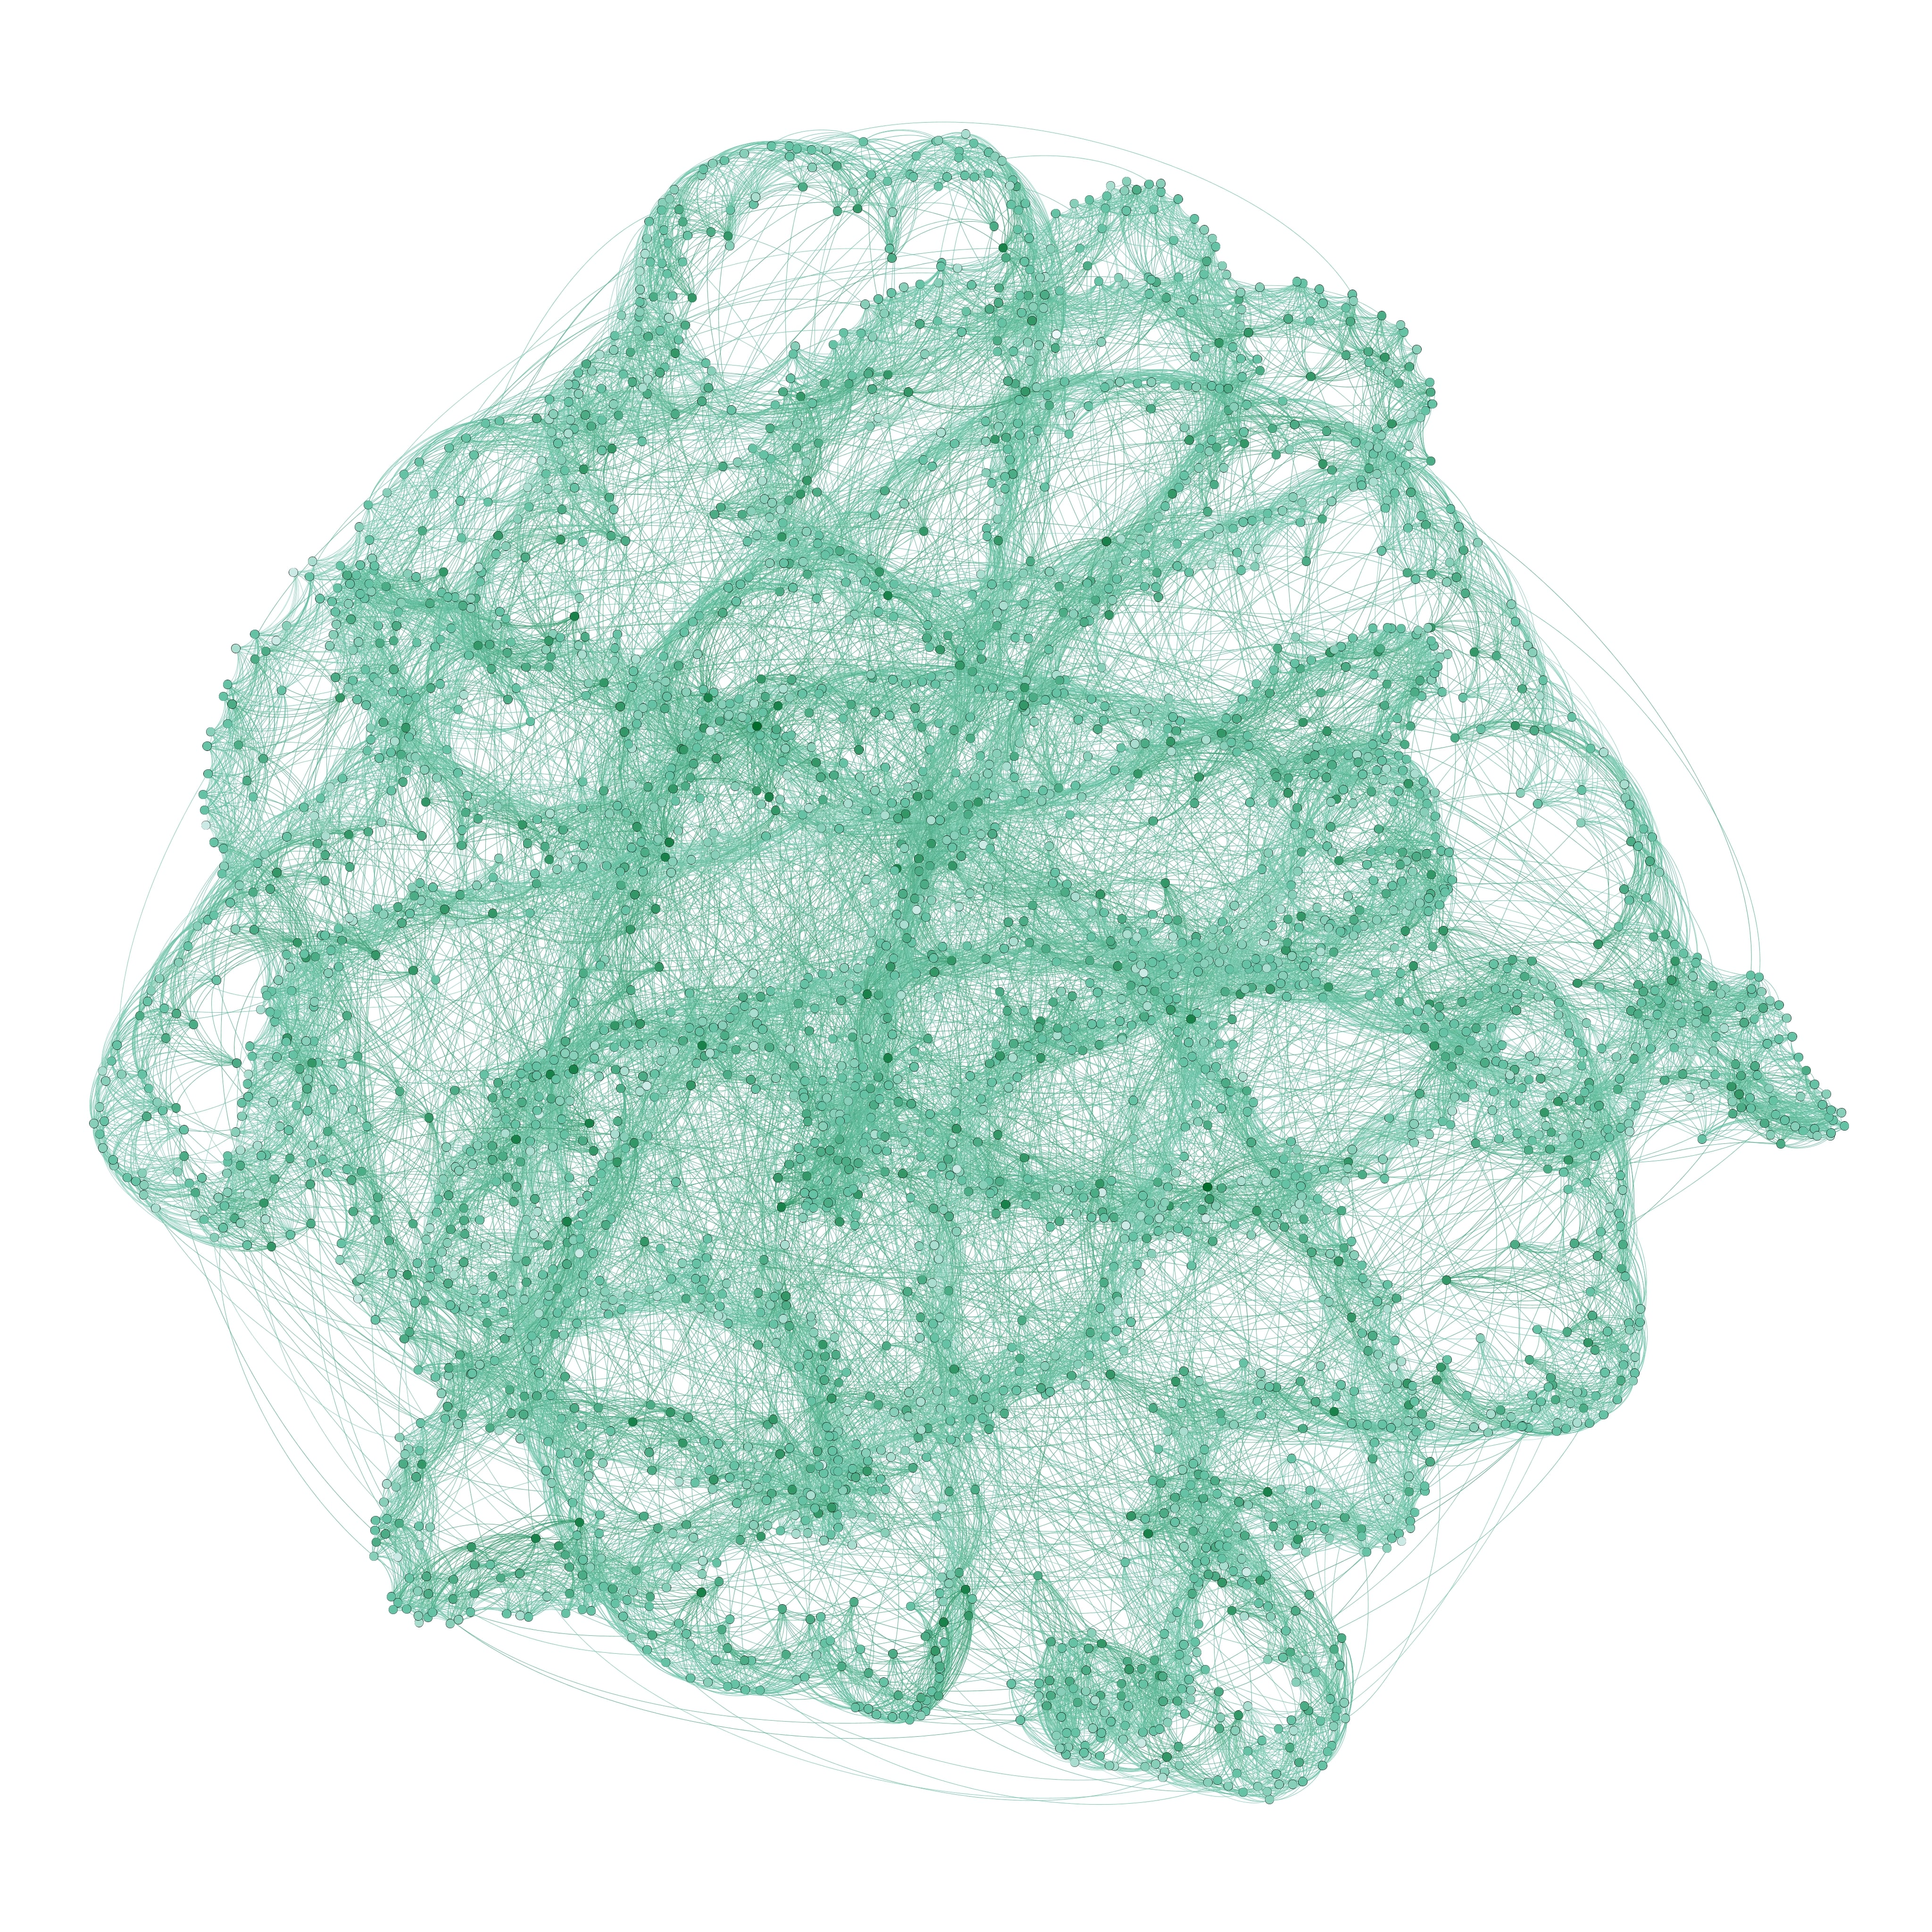
\includegraphics[width=\textwidth]{4b_small_world}
\caption{Small World Network n=3035,k=25,p=0.05} \label{fig_4_smallworld}
\end{figure}


\begin{figure}
    \centering
    \begin{minipage}{0.5\textwidth}
        \centering
        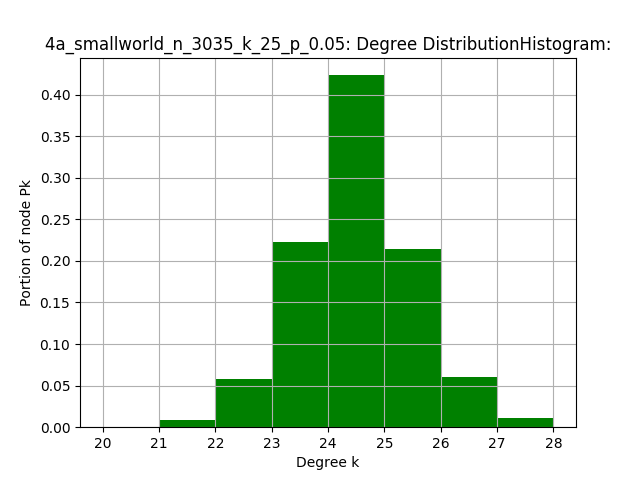
\includegraphics[width=\textwidth]{4b_sw_dedist}
        \caption{Degree Distribution}
        \label{fig_4b_sw_degreedist_hist}
    \end{minipage}\hfill
    \begin{minipage}{0.5\textwidth}
        \centering
        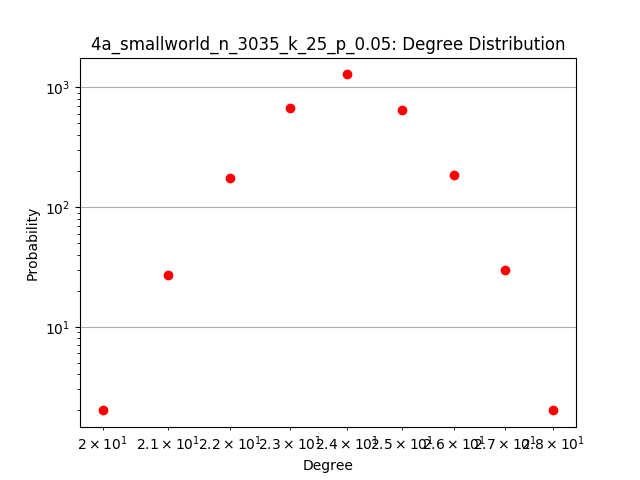
\includegraphics[width=\textwidth]{4b_sw_dedist_log}
        \caption{Degree Distribution in log}
        \label{fig_4b_sw_degreedist_log}
    \end{minipage}
\end{figure}


\begin{figure}
    \centering
    \begin{minipage}{0.5\textwidth}
        \centering
        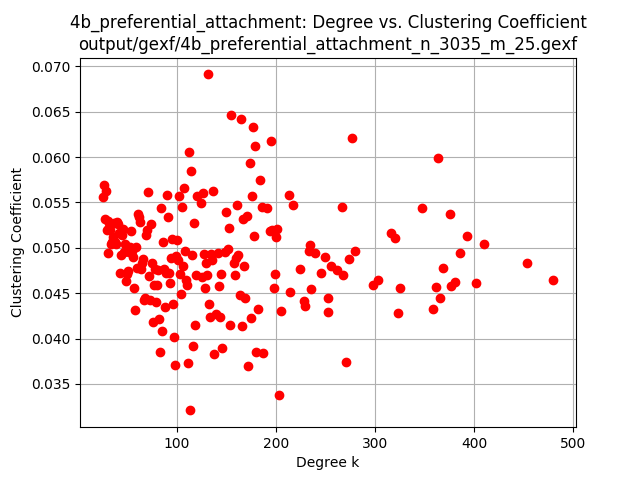
\includegraphics[width=\textwidth]{4b_preferential_attachment_clustering_coeff}
        \caption{Cluster. Coeff}
        \label{fig_4b_sw_clustering_coeff}
    \end{minipage}\hfill
    \begin{minipage}{0.5\textwidth}
        \centering
        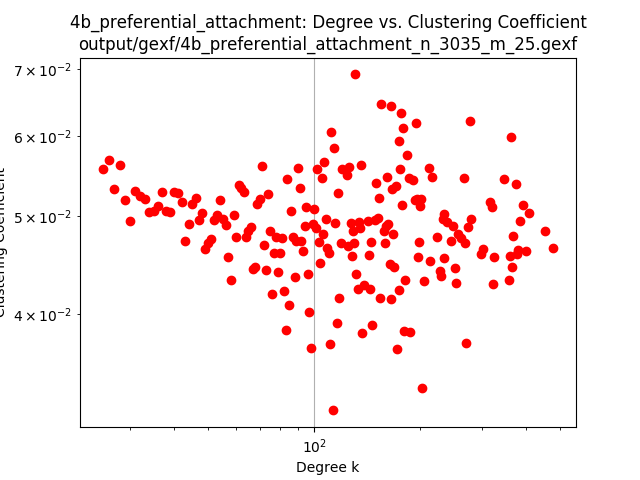
\includegraphics[width=\textwidth]{4b_preferential_attachment_clustering_coeff_log}
        \caption{ Cluster. Coeff in log}
        \label{fig_4b_sw_clustering_coeff_log}
    \end{minipage}
\end{figure}





For preferential attachment, I used Barabási-Albert model to construct.  I set the node size \(N = 3035\) and expected degree \( m =25 \). In the hope of generating similar average degree as player network, the expected degree is chose to be the half of average degree. 

Table.~\ref{tab_prefere_attach} shows the structural metrics of preferential attachment network. The average degree is almost the same as the player network. Both the average path length and clustering coefficient are much lower than that of original network. The clustering coefficient is around 0.05, lower by an order. This makes sense since new nodes have a preferential to attach to high degree nodes. The average path length is shortened due to big hubs. From the Fig.~\ref{fig_4b_perferrential}, we can observe several visible big hubs.

	Moreover, the clustering coefficient are shown in Fig.~\ref{fig_4b_preferential_attachment_clustering_coeff} and  Fig.~\ref{fig_4b_preferential_attachment_clustering_coeff_log}. With preferential attachment, the clustering coefficient is equally small for every node regardless of degree. 
 The degree distributions are shown in Fig.~\ref{fig_4b_pa_degreedist_hist} and  Fig.~\ref{fig_4b_pa_degreedist_log}. The distribution follows a power-law distribution and resembles that of player network.

\begin{table}
\centering
\caption{Structural Metrics of Preferential Attachment network.}\label{tab_prefere_attach}
\begin{tabular}{|l|l|}
\hline
metric & value \\
\hline
average degree & 49.58 \\
order & 3035 \\
size & 75250 \\
density & 0.016344 \\
diameter & 3 \\
radius & 2 \\
average path length & 2.355214 \\
average clustering coefficient & 0.051652 \\
transitivity & 0.049413 \\
number of triangle & 108398 \\ 
number of clique & 80531 \\
number of component & 1 \\ \hline
\end{tabular}
\end{table}

\begin{figure}
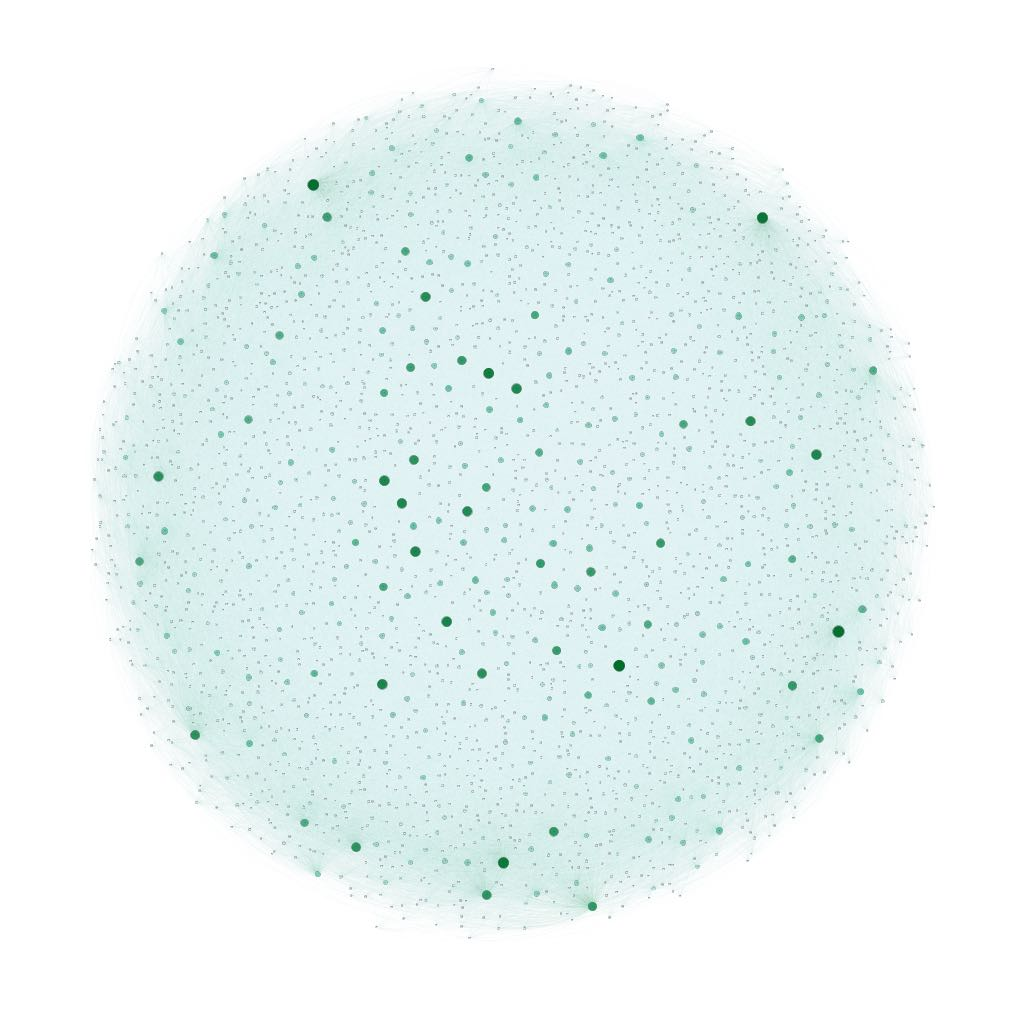
\includegraphics[width=\textwidth]{4b_perferrential}
\caption{Perferential Attachment n=3035,m=25} \label{fig_4b_perferrential}
\end{figure}


\begin{figure}
    \centering
    \begin{minipage}{0.5\textwidth}
        \centering
        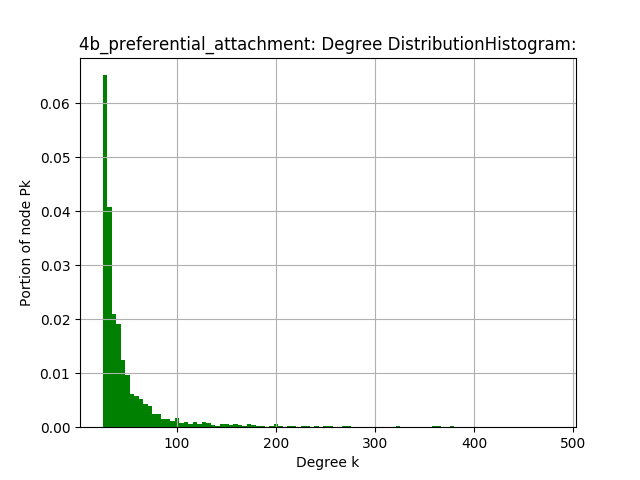
\includegraphics[width=\textwidth]{4b_preferential_attachment_Degree_dist_hist} % first figure itself
        \caption{Degree Distribution}
        \label{fig_4b_pa_degreedist_hist}
    \end{minipage}\hfill
    \begin{minipage}{0.5\textwidth}
        \centering
        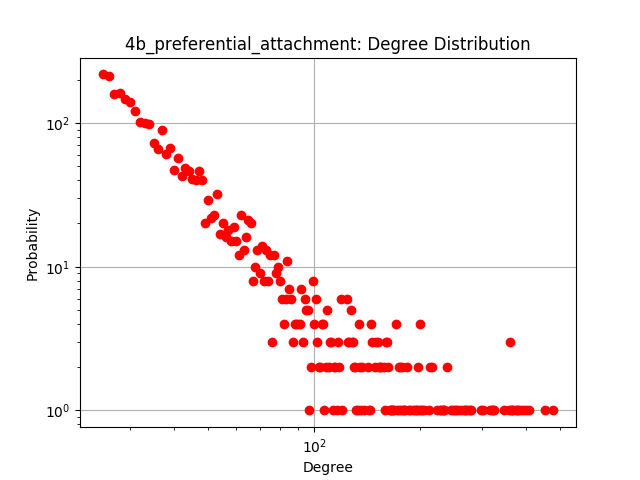
\includegraphics[width=\textwidth]{4b_preferential_attachment_Degree_dist_log} % second figure itself
        \caption{Degree Distribution in log}
        \label{fig_4b_pa_degreedist_log}
    \end{minipage}
\end{figure}


\begin{figure}
    \centering
    \begin{minipage}{0.5\textwidth}
        \centering
        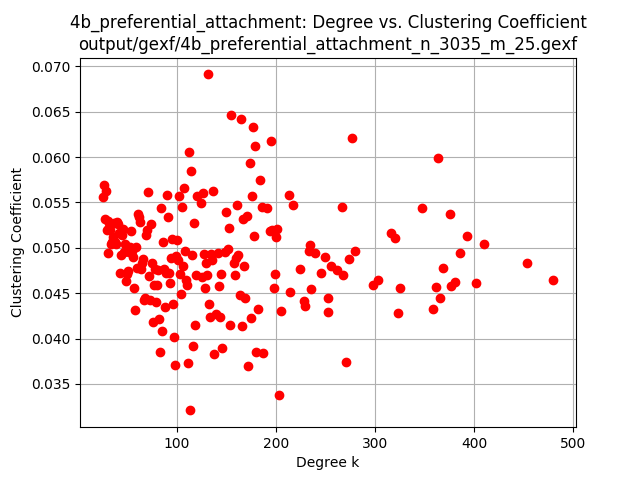
\includegraphics[width=\textwidth]{4b_preferential_attachment_clustering_coeff} % first figure itself
        \caption{Cluster. Coeff}
        \label{fig_4b_preferential_attachment_clustering_coeff}
    \end{minipage}\hfill
    \begin{minipage}{0.5\textwidth}
        \centering
        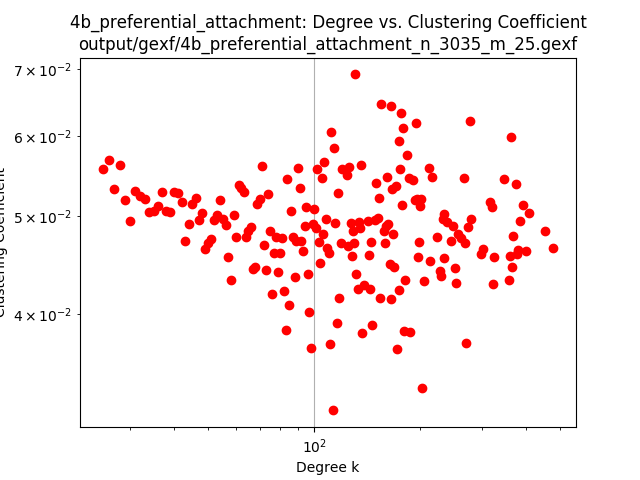
\includegraphics[width=\textwidth]{4b_preferential_attachment_clustering_coeff_log} % second figure itself
        \caption{ Cluster. Coeff in log}
        \label{fig_4b_preferential_attachment_clustering_coeff_log}
    \end{minipage}
\end{figure}

Looking further in to the scale-freeness of both preferential attachment and player network, we are able to approximate scale-freeness \( \alpha \) with following formula:
\begin{math}
	k_{max} = k_{min}N^\frac{1}{\alpha -1}
\end{math}.

The comparison of scale-free is shown in Table~\ref{tab_free_scale_compare}. The \(\alpha\) of preferential attachment is 3.71 and player network is 2.11. From the Fig.~\ref{fig_4b_degree_dist_compare_log}, both the degree distributions are shown in log scale. Indeed the slope of preferential attachment is almost twice of player network. In the lecture, it is told that a network enters scale free regime with \(\alpha\) between 2 and 3. Judging from the degree distribution, I can say that both of the networks are scale-free. Therefore, player network is close to preferential attachment network. 

\begin{table}
\centering
\caption{Free-Scale Compare} \label{tab_free_scale_compare}
\begin{tabular}{|l|l|l|}
\hline
parameter & preferential  & player  \\
&  network &  network \\ \hline
\(\alpha\) & 3.71 & 2.11 \\ 
k_{max} & 480 & 1290 \\ 
k_{min} & 25 & 1 \\ 
N & 3035 & 3035 \\ \hline

\end{tabular}
\end{table}

\begin{figure} [H]
\centering
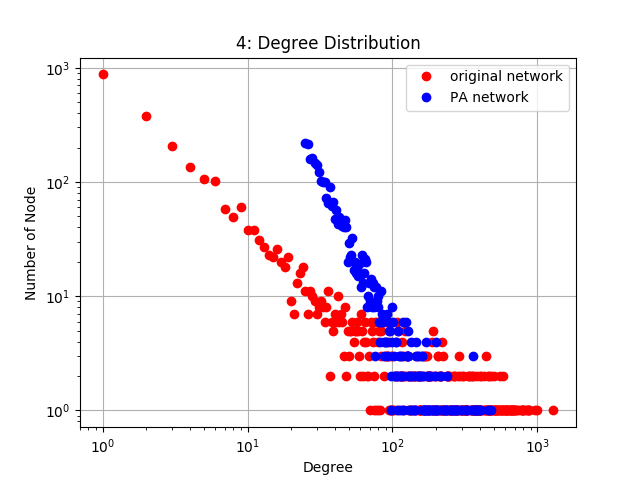
\includegraphics[width=\textwidth]{4_degree_dist_compare_log}
\caption{Degree Dist. Comparison} \label{fig_4b_degree_dist_compare_log}
\end{figure}


\section{Conclusions and Outlook}

In this project, I have constructed a tennis player network based on match statistics. I analyzed the player network in terms of structural metrics, centralities, and network model. After comparing 6 top 10 different centralities, I reached a conclusion that Katz centrality performs best rank for player evaluation. In network model comparison,  player network exhibits scale-free model with \(\alpha\) approximating 2.1. 
We can see that simple graphical analysis on network already gives insights for tennis player evaluation. By adding more attributes in the network, we will be able to answer question such as which of them is better n serving, tiebreak, returning or winning-rate. New rankings for tennis can be explored through further investigation.
%
% ---- Bibliography ----
%
\bibliographystyle{splncs04}
\bibliography{mybib}
All links were last followed on January 30, 2020.

\end{document}
